%%%%%%%%%%%%%%%%%%%%%%%%%%%%%%%%%%%%%%%%%%%%%%%%%%%%%%%%%%%%%%%%%%%%%%%%%%%%%%%%%%
\begin{frame}[fragile]\frametitle{}
\begin{center}
{\Large Q Learning}
\end{center}
\end{frame}


%%%%%%%%%%%%%%%%%%%%%%%%%%%%%%%%%%%%%%%%%%%%%%%%%%%%%%%%%%%%%%%%%%%%%%%%%%%%%%%%%%
\begin{frame}[fragile]\frametitle{Approaches for solving RL problems}

\begin{itemize}
\item how do we solve the RL problem?
\item In other terms, how to build an RL agent that can select the actions that maximize its expected cumulative reward?
\end{itemize}

{\tiny (Ref: Chapter 1 of the Deep Reinforcement Learning Class with Hugging Face)}


\end{frame}

%%%%%%%%%%%%%%%%%%%%%%%%%%%%%%%%%%%%%%%%%%%%%%%%%%%%%%%%%%%%%%%%%%%%%%%%%%%%%%%%%%
\begin{frame}[fragile]\frametitle{The Policy $\pi$}


\begin{itemize}
\item The Policy $\pi$: the agent’s brain
\item It’s the function that tell us what action to take given the state we are. So it defines the agent’s behavior at a given time.
\item This Policy is the function we want to learn, our goal is to find the optimal policy $\pi^*$, the policy that  maximizes expected return when the agent acts according to it. We find this $\pi$ through training.
\end{itemize}

{\tiny (Ref: Chapter 1 of the Deep Reinforcement Learning Class with Hugging Face)}


\end{frame}

%%%%%%%%%%%%%%%%%%%%%%%%%%%%%%%%%%%%%%%%%%%%%%%%%%%%%%%%%%%%%%%%%%%%%%%%%%%%%%%%%%
\begin{frame}[fragile]\frametitle{Optimal policy $\pi^*$}

There are two approaches to train our agent to find this optimal policy  $\pi^*$:

\begin{itemize}
\item Directly, by teaching the agent to learn which action to take, given the state is in: Policy-Based Methods.
\item Indirectly, teach the agent to learn which state is more valuable and then take the action that leads to the more valuable states: Value-Based Methods.
\end{itemize}

\begin{center}
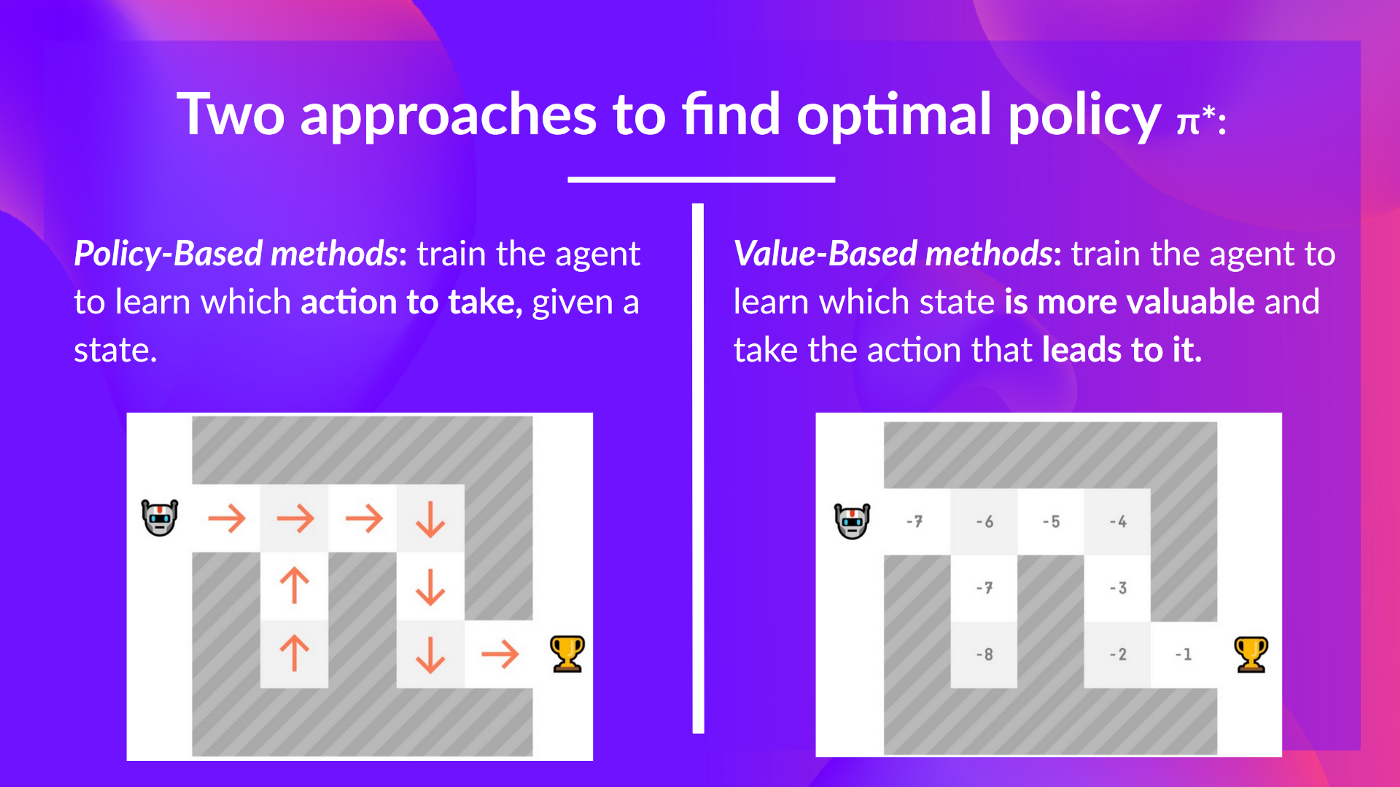
\includegraphics[width=0.8\linewidth,keepaspectratio]{rl101}
\end{center}



{\tiny (Ref: Chapter 1 of the Deep Reinforcement Learning Class with Hugging Face)}


\end{frame}

%%%%%%%%%%%%%%%%%%%%%%%%%%%%%%%%%%%%%%%%%%%%%%%%%%%%%%%%%%%%%%%%%%%%%%%%%%%%%%%%%%
\begin{frame}[fragile]\frametitle{Policy-Based Methods}

\begin{itemize}
\item In Policy-Based Methods, we learn a policy function directly.
\item This function will map from each state to the best corresponding action at that state. Or a probability distribution over the set of possible actions at that state.
\item  In this case, we don't have a value function.
\item And consequently, we don't define by hand the behavior of our policy; it's the training that will define it.
\end{itemize}

We have two types of policy:
\begin{itemize}
\item Deterministic: a policy at a given state will always return the same action.
\item Stochastic: output a probability distribution over actions.
\end{itemize}

{\tiny (Ref: Chapter 1 of the Deep Reinforcement Learning Class with Hugging Face)}


\end{frame}

%%%%%%%%%%%%%%%%%%%%%%%%%%%%%%%%%%%%%%%%%%%%%%%%%%%%%%%%%%%%%%%%%%%%%%%%%%%%%%%%%%
\begin{frame}[fragile]\frametitle{Value-based methods}

\begin{itemize}
\item Indirectly, by training a value function that outputs the value of a state or a state-action pair. Given this value function, our policy will take action.
\item In Value-based methods, instead of training a policy function, we train a value function that maps a state to the expected value of being at that state.
\item But, because we didn't train our policy, we need to specify its behavior. For instance, if we want a policy that, given the value function, will take actions that always lead to the biggest reward, we'll create a Greedy Policy.
\item The value of a state is the expected discounted return the agent can get if it starts in that state, and then act according to our policy. ``Act according to our policy'' just means that our policy is “going to the state with the highest value”.
\item At the end of learning, value function defines value for each possible state.
\item Thanks to our value function, at each step our policy will select the state with the biggest value defined by the value function
\end{itemize}


{\tiny (Ref: Chapter 1 of the Deep Reinforcement Learning Class with Hugging Face)}


\end{frame}


%%%%%%%%%%%%%%%%%%%%%%%%%%%%%%%%%%%%%%%%%%%%%%%%%%%%%%%%%%%%%%%%%%%%%%%%%%%%%%%%%%
\begin{frame}[fragile]\frametitle{The ``Deep'' in Reinforcement Learning}

\begin{itemize}
\item We can use a traditional algorithm to create a Q table that helps us find what action to take for each state, ok for small number of states
\item For bigger and complex problems, we use a Neural Network (to approximate the q value).
\end{itemize}


{\tiny (Ref: Chapter 1 of the Deep Reinforcement Learning Class with Hugging Face)}


\end{frame}

%%%%%%%%%%%%%%%%%%%%%%%%%%%%%%%%%%%%%%%%%%%%%%%%%%%%%%%%%%%%%%%%%%%%%%%%%%%%%%%%%%
\begin{frame}[fragile]\frametitle{Find Optimal Policy}

Consequently, whatever method you use to solve your problem, you will have a policy, but in the case of value-based methods you don't train it, your policy is just a simple function that you specify (for instance greedy policy) and this policy uses the values given by the value-function to select its actions.

So the difference is:
\begin{itemize}
\item In policy-based, the optimal policy is found by training the policy directly.
\item In value-based, finding an optimal value function leads to having an optimal policy.
\end{itemize}

In fact, most of the time, in value-based methods, you'll use an Epsilon-Greedy Policy that handles the exploration/exploitation trade-off.

{\tiny (Ref: Chapter 2/1 of the Deep Reinforcement Learning Class with Hugging Face)}


\end{frame}


%%%%%%%%%%%%%%%%%%%%%%%%%%%%%%%%%%%%%%%%%%%%%%%%%%%%%%%%%%%%%%%%%%%%%%%%%%%%%%%%%%
\begin{frame}[fragile]\frametitle{Types of Value-based functions}

The two types of value-based functions:

\begin{itemize}
\item The State-Value function: For each state, the state-value function outputs the expected return if the agent starts at that state, and then follow the policy forever after (for all future timesteps if you prefer).
\item The Action-Value function: For each state and action pair, the action-value function outputs the expected return if the agent starts in that state and takes action, and then follows the policy forever after.
\item So, the difference is:
	\begin{itemize}
	\item In state-value function, we calculate the value of a state $S_t$
	\item In action-value function we calculate the value of the state action pair $(S_t, A_t)$ hence the value of taking that action that the state.
	\end{itemize}
\item In either case, whatever value function we choose (state-value or action-value function), the value is the expected return.
\item However, the problem is that it implies that to calculate EACH value of a state or a state-action pair, we need to sum all the rewards an agent can get if it starts at that state.
\item This can be a tedious process, and that's where the Bellman equation comes to help us.
\end{itemize}




{\tiny (Ref: Chapter 1 of the Deep Reinforcement Learning Class with Hugging Face)}


\end{frame}

%%%%%%%%%%%%%%%%%%%%%%%%%%%%%%%%%%%%%%%%%%%%%%%%%%%%%%%%%%%%%%%%%%%%%%%%%%%%%%%%%%
\begin{frame}[fragile]\frametitle{The Bellman Equation}


\begin{itemize}
\item The Bellman equation simplifies our state value or state-action value calculation.
\item if we calculate the $V(S_t)$ (value of a state), we need to calculate the return starting at that state and then follow the policy forever after. (Our policy that we defined in the following example is a Greedy Policy, and for simplification, we don't discount the reward).
\item Then, to calculate the $V(S_{t+1})$ we need to calculate the return starting at that state $S_{t+1}$. That's a pretty tedious process if you need to do it for each state value or state-action value. Use Bellman Equation.
\item The Bellman equation is a recursive equation that works like this: instead of starting for each state from the beginning and calculating the return, we can consider the value of any state as: The immediate reward $R_{t+1} +$ the discounted value of the state that follows $( gamma * V(S_{t+1}))$
\item To recap, the idea of the Bellman equation is that instead of calculating each value as the sum of the expected return, which is a long process. This is equivalent to the sum of immediate reward + the discounted value of the state that follows.
\end{itemize}


{\tiny (Ref: Chapter 1 of the Deep Reinforcement Learning Class with Hugging Face)}


\end{frame}


%%%%%%%%%%%%%%%%%%%%%%%%%%%%%%%%%%%%%%%%%%%%%%%%%%%%%%%%%%%%%%%%%%%%%%%%%%%%%%%%%%
\begin{frame}[fragile]\frametitle{Two Ways of Learning}


\begin{itemize}
\item Monte Carlo and Temporal Difference Learning are two different strategies on how to train our value function or our policy function. Both of them use experience to solve the RL problem.
\item Monte Carlo uses an entire episode of experience before learning ie learning at the end of the episode
\item Temporal Difference uses only a step $( S_t, A_t, R_{t+1}, S_{t+1})$ to learn.
\end{itemize}


{\tiny (Ref: Chapter 1 of the Deep Reinforcement Learning Class with Hugging Face)}


\end{frame}

%%%%%%%%%%%%%%%%%%%%%%%%%%%%%%%%%%%%%%%%%%%%%%%%%%%%%%%%%%%%%%%%%%%%%%%%%%%%%%%%%%
\begin{frame}[fragile]\frametitle{Monte Carlo}


\begin{itemize}
\item Monte Carlo waits until the end of the episode, calculates $G_t$ (return) and uses it as a target for updating $V(S_t)$.
\item So it requires a complete entire episode of interaction before updating our value function.
\end{itemize}

{\tiny (Ref: Chapter 1 of the Deep Reinforcement Learning Class with Hugging Face)}


\end{frame}

%%%%%%%%%%%%%%%%%%%%%%%%%%%%%%%%%%%%%%%%%%%%%%%%%%%%%%%%%%%%%%%%%%%%%%%%%%%%%%%%%%
\begin{frame}[fragile]\frametitle{Monte Carlo Process}


\begin{center}
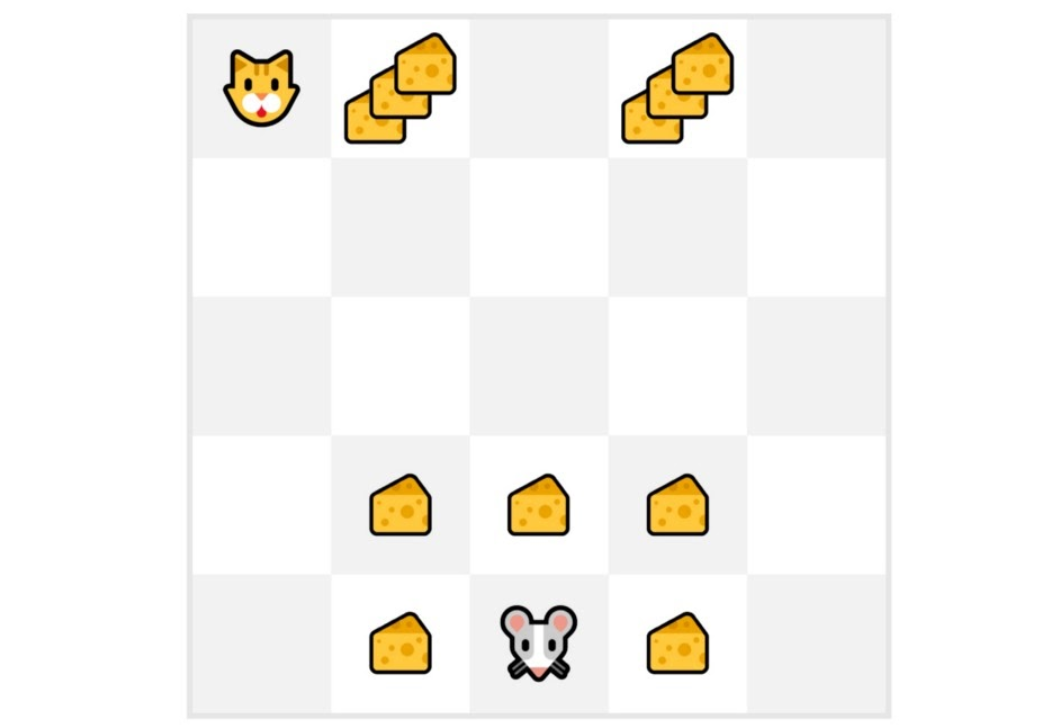
\includegraphics[width=0.4\linewidth,keepaspectratio]{rl110}
\end{center}


\begin{itemize}
\item We always start the episode at the same starting point.
\item The agent takes actions using the policy. For instance, using an Epsilon Greedy Strategy, a policy that alternates between exploration (random actions) and exploitation.
\item We get the reward and the next state.
\item We terminate the episode if the cat eats the mouse or if the mouse moves $> 10$ steps.
\item At the end of the episode, we have a list of State, Actions, Rewards, and Next States
\item  The agent will sum the total rewards $G_t$ (to see how well it did).
\item It will then update $V(s_t)$ based on the formula $V(S_t) \leftarrow V(S_t) + \alpha [ G_t - V(S_t)]$
\item Then start a new game with this new knowledge
\item By running more and more episodes, the agent will learn to play better and better.
\end{itemize}


{\tiny (Ref: Chapter 1 of the Deep Reinforcement Learning Class with Hugging Face)}

\end{frame}


%%%%%%%%%%%%%%%%%%%%%%%%%%%%%%%%%%%%%%%%%%%%%%%%%%%%%%%%%%%%%%%%%%%%%%%%%%%%%%%%%%
\begin{frame}[fragile]\frametitle{Monte Carlo Process}

For instance, if we train a state-value function using Monte Carlo:

\begin{center}
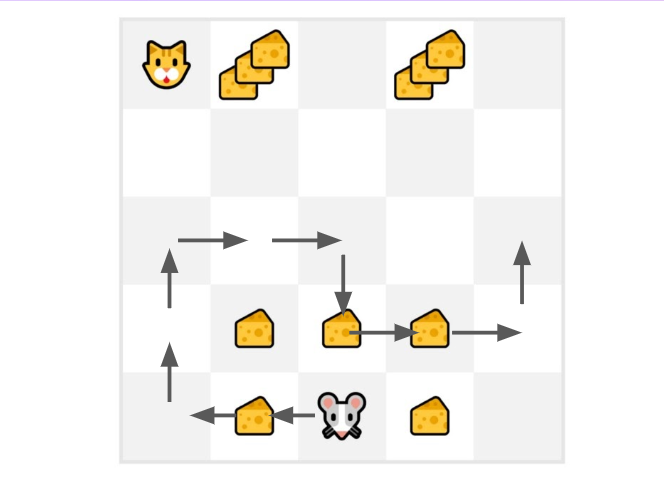
\includegraphics[width=0.4\linewidth,keepaspectratio]{rl111}
\end{center}


\begin{itemize}
\item We just started to train our Value function, so it returns 0 value for each state
\item Our learning rate (lr) is 0.1 and our discount rate is 1 (= no discount)
\item Our mouse explores the environment and takes random actions
\item The mouse made more than 10 steps, so the episode ends .
\item We have a list of state, action, rewards, next\_state, we need to calculate the return $G_{t}$
\item $G_t = R_{t+1} + R_{t+2} + R_{t+3} + \ldots $ (no discounting)
\item $G_t = 1 + 0 + 0 + 1 + 1 + 0 + \ldots$
\item $G_t = 3$
\item We can now update $V(S_0)$ as $V(S_t) \leftarrow V(S_t) + \alpha [ G_t - V(S_t)]$
\item $V(S_0) \leftarrow 0 + 0.1 * [3 - 0]$
\item $V(S_0) = 0.3$
\end{itemize}


{\tiny (Ref: Chapter 1 of the Deep Reinforcement Learning Class with Hugging Face)}

\end{frame}



%%%%%%%%%%%%%%%%%%%%%%%%%%%%%%%%%%%%%%%%%%%%%%%%%%%%%%%%%%%%%%%%%%%%%%%%%%%%%%%%%%
\begin{frame}[fragile]\frametitle{Temporal Difference Learning}

Learning at each step

\begin{itemize}
\item Temporal difference, on the other hand, waits for only one interaction (one step) $S_{t+1}$ to form a TD target and update $V(S_t)$ using $R_{t+1}$ and $gamma * V(S_{t+1})$.
\item The idea with TD is to update the $V(S_t)$ at each step.
\item But because we didn't play during an entire episode, we don't have $G_t$ (expected return). Instead, we estimate $G_t$ by adding $R_{t+1}$ and the discounted value of the next state.
\item We speak about bootstrap because TD bases its update part on an existing estimate $V(S_{t+1})$ and not a complete sample $G_t$.
\item This method is called $TD(0)$ or one-step TD (update the value function after any individual step).

\end{itemize}


{\tiny (Ref: Chapter 1 of the Deep Reinforcement Learning Class with Hugging Face)}

\end{frame}

%%%%%%%%%%%%%%%%%%%%%%%%%%%%%%%%%%%%%%%%%%%%%%%%%%%%%%%%%%%%%%%%%%%%%%%%%%%%%%%%%%
\begin{frame}[fragile]\frametitle{Temporal Difference Process}

For instance, if we train a state-value function using Temporal Difference:

\begin{center}
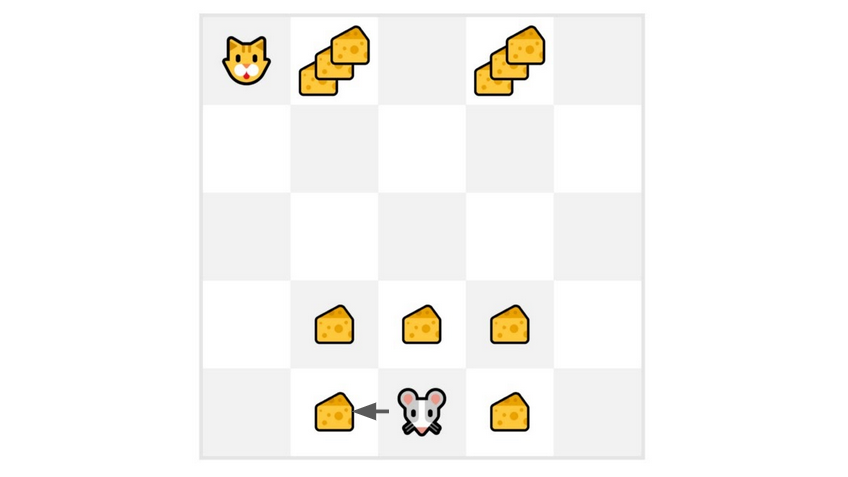
\includegraphics[width=0.4\linewidth,keepaspectratio]{rl112}
\end{center}


\begin{itemize}
\item We just started to train our Value function, so it returns 0 value for each state.
\item Our learning rate (lr) is 0.1, and our discount rate is 1 (no discount).
\item Our mouse explore the environment and take a random action: going to the left
\item It gets a reward $R_{t+1} = 1$ since it eats a piece of cheese
\item We can now update $V(S_0)$ by $V(S_t)$ using $R_{t+1}$ and $gamma * V(S_{t+1})$.
\item $V(S_0) = V(S_0) + \alpha * [R_{0+1} + \gamma * V(S_{0+1}) -V(S_0)] $.
\item $V(S_0) = 0 + 0.1 * [1 + 1 * 0 - 0] = 0.1$.
\item So we just updated our value function for State 0.
\item Now we continue to interact with this environment with our updated value function.
\end{itemize}


{\tiny (Ref: Chapter 1 of the Deep Reinforcement Learning Class with Hugging Face)}

\end{frame}



%%%%%%%%%%%%%%%%%%%%%%%%%%%%%%%%%%%%%%%%%%%%%%%%%%%%%%%%%%%%%%%%%%%%%%%%%%%%%%%%%%
\begin{frame}[fragile]\frametitle{Summary}


\begin{itemize}
\item With Monte Carlo, we update the value function from a complete episode, and so we use the actual accurate discounted return of this episode.
\item With TD learning, we update the value function from a step, so we replace $G_t$ that we don't have with an estimated return called TD target.
\end{itemize}


\begin{center}
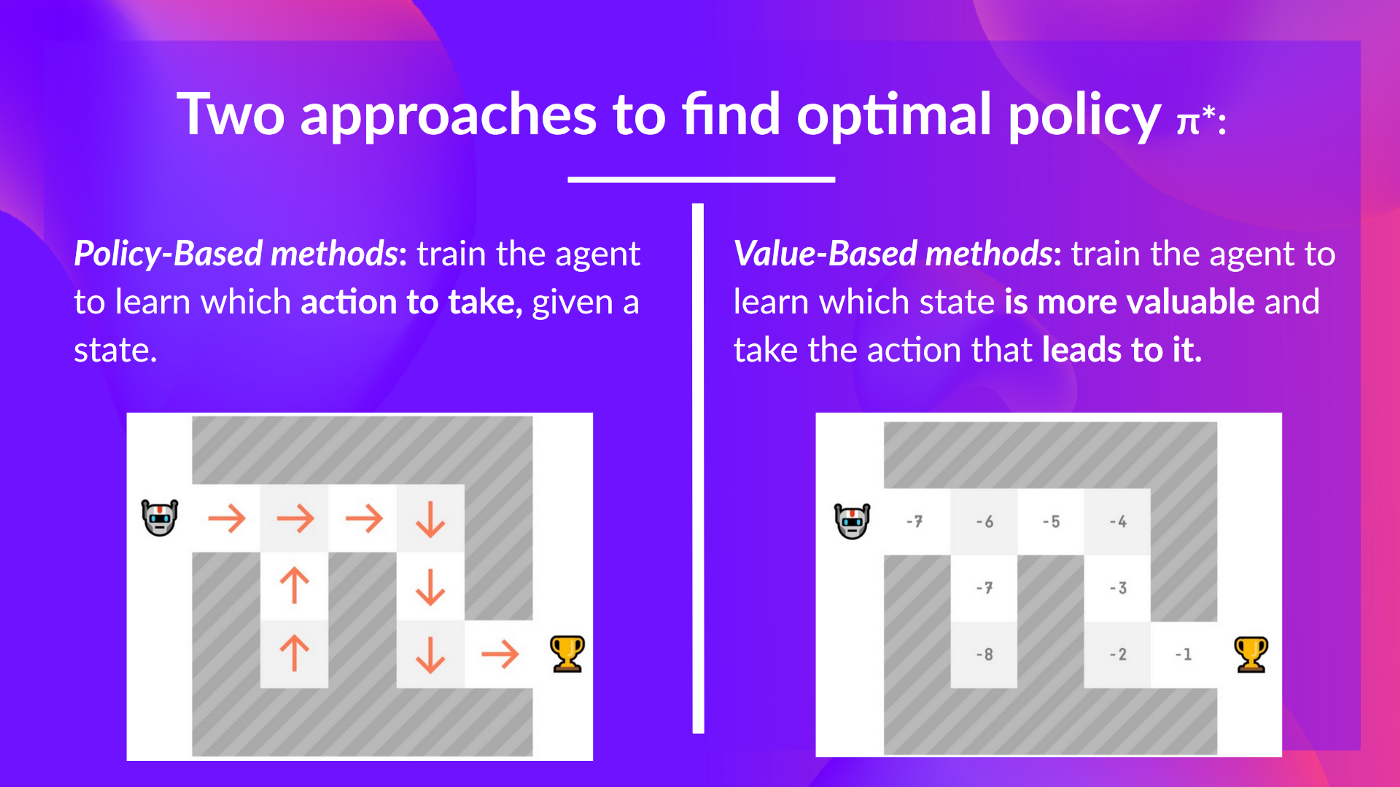
\includegraphics[width=0.8\linewidth,keepaspectratio]{rl101}
\end{center}



{\tiny (Ref: Chapter 1 of the Deep Reinforcement Learning Class with Hugging Face)}

\end{frame}


%%%%%%%%%%%%%%%%%%%%%%%%%%%%%%%%%%%%%%%%%%%%%%%%%%%%%%%%%%%%%%%%%%%%%%%%%%%%%%%%%%
\begin{frame}[fragile]\frametitle{What is Q-Learning?}

\begin{itemize}

\item Q-Learning is an off-policy value-based method that uses a TD approach to train its action-value function:


\begin{itemize}
\item Off-policy (?)
\item Value-based method: finds the optimal policy indirectly by training a value or action-value function that will tell us the value of each state or each state-action pair.
\item Uses a TD approach: updates its action-value function at each step instead of at the end of the episode.
\end{itemize}

\item Given a state and action, our Q Function outputs a state-action value (also called Q-value)
\item The Q comes from "the Quality" of that action at that state.
\item Q-Learning is the algorithm we use to train our Q-Function, an action-value function that determines the value of being at a particular state and taking a specific action at that state.
\item Internally, our Q-function has a Q-table, a table where each cell corresponds to a state-action value pair value. Think of this Q-table as the memory or cheat sheet of our Q-function.
\end{itemize}


If we take this maze example:
\begin{center}
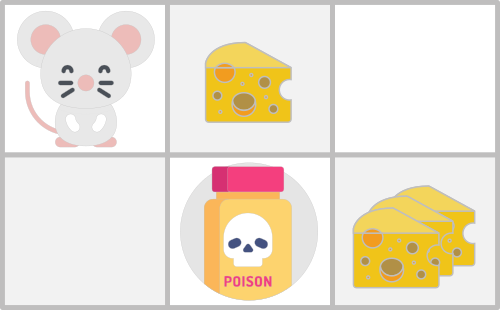
\includegraphics[width=0.4\linewidth,keepaspectratio]{rl113}
\end{center}

Therefore, Q-function contains a Q-table that has the value of each-state action pair. And given a state and action, our Q-Function will search inside its Q-table to output the value.

{\tiny (Ref: Chapter 2 of the Deep Reinforcement Learning Class with Hugging Face)}

\end{frame}

%%%%%%%%%%%%%%%%%%%%%%%%%%%%%%%%%%%%%%%%%%%%%%%%%%%%%%%%%%%%%%%%%%%%%%%%%%%%%%%%%%
\begin{frame}[fragile]\frametitle{The Q-Learning algorithm}


\begin{center}
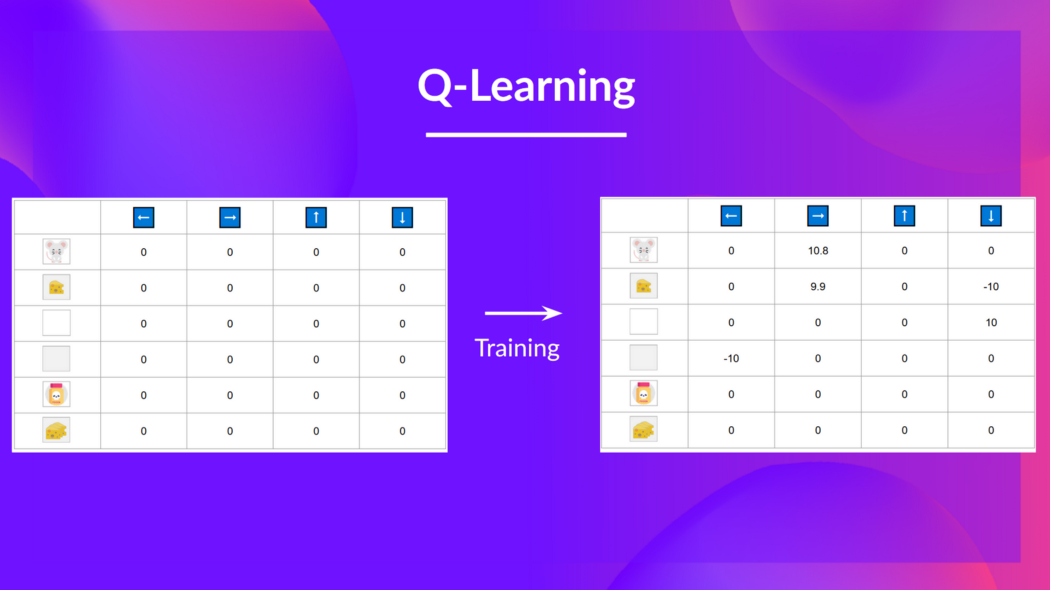
\includegraphics[width=0.8\linewidth,keepaspectratio]{rl116}
\end{center}

{\tiny (Ref: Chapter 3 of the Deep Reinforcement Learning Class with Hugging Face)}

\end{frame}

%%%%%%%%%%%%%%%%%%%%%%%%%%%%%%%%%%%%%%%%%%%%%%%%%%%%%%%%%%%%%%%%%%%%%%%%%%%%%%%%%%
\begin{frame}[fragile]\frametitle{The Q-Learning algorithm}

\begin{itemize}
\item Step 1: We initialize the Q-Table, say , with 0
\item Step 2: Choose action using Epsilon Greedy Strategy.  define $\epsilon = 1.0$:
\begin{itemize}
\item With probability $1 — \epsilon$ : we do exploitation (aka our agent selects the action with the highest state-action pair value).
\item With probability $\epsilon$: we do exploration (trying random action). 
\end{itemize}
\item At the beginning of the training, the probability of doing exploration will be huge since $\epsilon$ is very high, so most of the time, we'll explore. But as the training goes on, and consequently our Q-Table gets better and better in its estimations, we progressively reduce the epsilon value since we will need less and less exploration and more exploitation.
\item Step 3: Perform action $A_t$, gets reward $R_{t+1}$ and next state $S_{t+1}$
\item Step 4: Update $Q(S_t, A_t)$. Remember that in TD Learning, we update our policy or value function (depending on the RL method we choose) after one step of the interaction.
\item To produce our TD target, we used the immediate reward $R_{t+1}$ plus the discounted value of the next state best state-action pair (we call that bootstrap).

\end{itemize}


\begin{center}
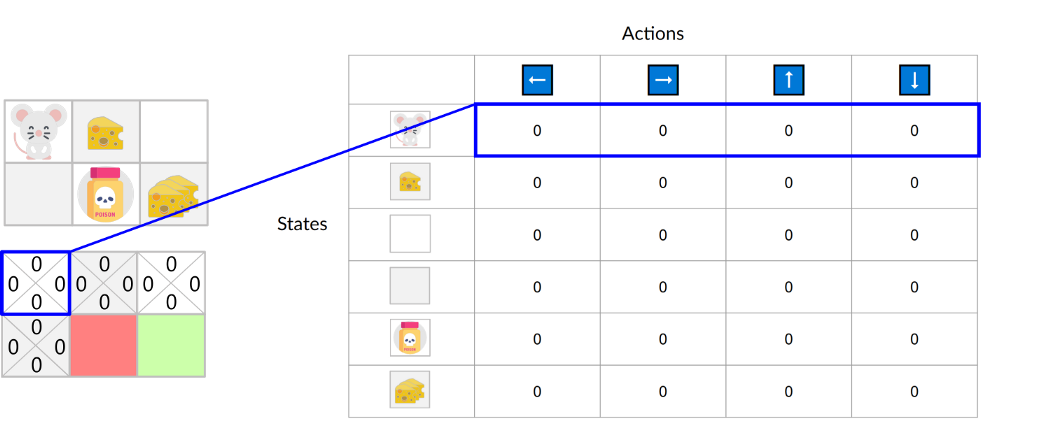
\includegraphics[width=0.8\linewidth,keepaspectratio]{rl114}
\end{center}

Therefore, our $Q(S_t, A_t)$ update formula goes like this:

\begin{center}
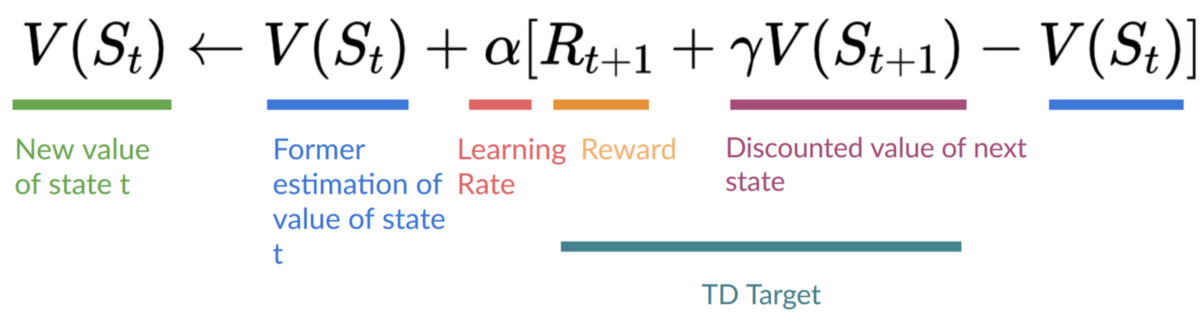
\includegraphics[width=0.8\linewidth,keepaspectratio]{rl104}
\end{center}

 
{\tiny (Ref: Chapter 2 of the Deep Reinforcement Learning Class with Hugging Face)}

\end{frame}

%%%%%%%%%%%%%%%%%%%%%%%%%%%%%%%%%%%%%%%%%%%%%%%%%%%%%%%%%%%%%%%%%%%%%%%%%%%%%%%%%%
\begin{frame}[fragile]\frametitle{The Q-Learning algorithm}

It means that to update our $Q(S_t, A_t)$:
\begin{itemize}
\item We need $S_t, A_t, R_{t+1}, S_{t+1}$.
\item To update our Q-value at a given state-action pair, we use the TD target.
\end{itemize}

How do we form the TD target?

\begin{itemize}
\item We obtain the reward after taking the action $R_{t+1}$.
\item To get the best next-state-action pair value, we use a greedy policy to select the next best action. Note that this is not an epsilon greedy policy, this will always take the action with the highest state-action value.
\end{itemize}

Then when the update of this Q-value is done. We start in a new\_state and select our action using our epsilon-greedy policy again.

It's why we say that this is an off-policy algorithm.

 
{\tiny (Ref: Chapter 2 of the Deep Reinforcement Learning Class with Hugging Face)}

\end{frame}

%%%%%%%%%%%%%%%%%%%%%%%%%%%%%%%%%%%%%%%%%%%%%%%%%%%%%%%%%%%%%%%%%%%%%%%%%%%%%%%%%%
\begin{frame}[fragile]\frametitle{Off-policy vs On-policy}

The difference is subtle:

\begin{itemize}
\item Off-policy: using a different policy for acting and updating. For instance, with Q-Learning, the Epsilon greedy policy (acting policy), is different from the greedy policy that is used to select the best next-state action value to update our Q-value (updating policy). Is different from the policy we use during the training part: $\gamma max_a Q(S_{t+1},a)$

\item On-policy: using the same policy for acting and updating. For instance, with Sarsa, another value-based algorithm, the Epsilon-Greedy Policy selects the next\_state-action pair, not a greedy policy.

\end{itemize}


{\tiny (Ref: Chapter 2 of the Deep Reinforcement Learning Class with Hugging Face)}

\end{frame}

%%%%%%%%%%%%%%%%%%%%%%%%%%%%%%%%%%%%%%%%%%%%%%%%%%%%%%%%%%%%%%%%%%%%%%%%%%%%%%%%%%
\begin{frame}[fragile]\frametitle{The Q-Learning algorithm}


\begin{center}
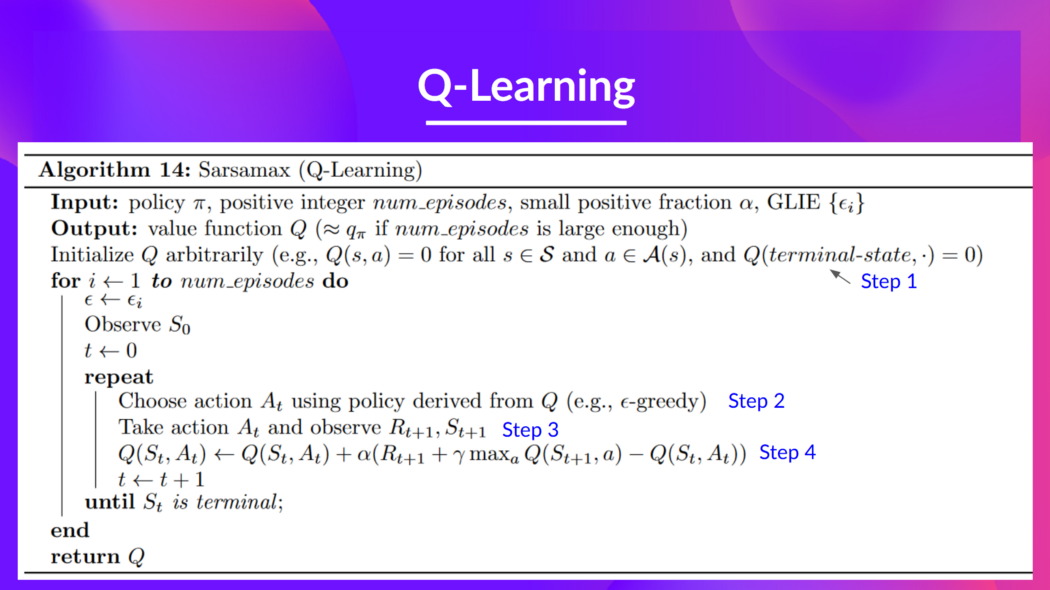
\includegraphics[width=0.8\linewidth,keepaspectratio]{rl103}
\end{center}

{\tiny (Ref: Chapter 2 of the Deep Reinforcement Learning Class with Hugging Face)}

\end{frame}

%%%%%%%%%%%%%%%%%%%%%%%%%%%%%%%%%%%%%%%%%%%%%%%%%%%%%%%%%%%%%%%%%%%%%%%%%%%%%%%%%%
\begin{frame}[fragile]\frametitle{The Q-Learning Example}


\begin{center}
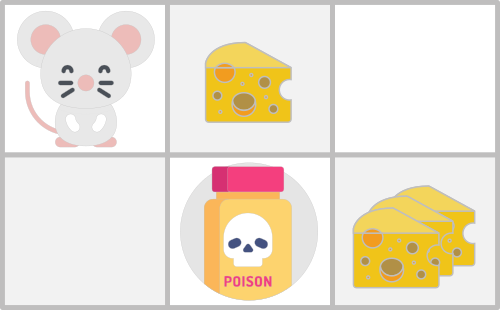
\includegraphics[width=0.4\linewidth,keepaspectratio]{rl113}
\end{center}

\begin{itemize}
\item You're a mouse in this tiny maze. You always start at the same starting point.
\item The goal is to eat the big pile of cheese at the bottom right-hand corner and avoid the poison. After all, who doesn't like cheese?
\item The episode ends if we eat the poison, eat the big pile of cheese or if we spent more than five steps.
\item The learning rate is 0.1
\item The gamma (discount rate) is 0.99
\end{itemize}

{\tiny (Ref: Chapter 3 of the Deep Reinforcement Learning Class with Hugging Face)}

\end{frame}

%%%%%%%%%%%%%%%%%%%%%%%%%%%%%%%%%%%%%%%%%%%%%%%%%%%%%%%%%%%%%%%%%%%%%%%%%%%%%%%%%%
\begin{frame}[fragile]\frametitle{The Q-Learning Example}


\begin{center}
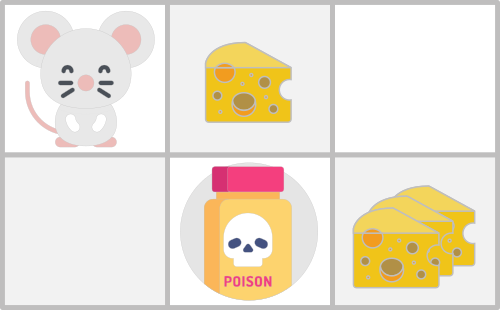
\includegraphics[width=0.4\linewidth,keepaspectratio]{rl113}
\end{center}

Reward function:

\begin{itemize}
\item +0: Going to a state with no cheese in it.
\item +1: Going to a state with a small cheese in it.
\item +10: Going to the state with the big pile of cheese.
\item -10: Going to the state with the poison and thus die.
\item +0 If we spend more than five steps.
\end{itemize}

To train our agent to have an optimal policy (so a policy that goes right, right, down), we will use the Q-Learning algorithm.


{\tiny (Ref: Chapter 3 of the Deep Reinforcement Learning Class with Hugging Face)}

\end{frame}

%%%%%%%%%%%%%%%%%%%%%%%%%%%%%%%%%%%%%%%%%%%%%%%%%%%%%%%%%%%%%%%%%%%%%%%%%%%%%%%%%%
\begin{frame}[fragile]\frametitle{The Q-Learning Example}

We initialize the Q-Table

\begin{center}
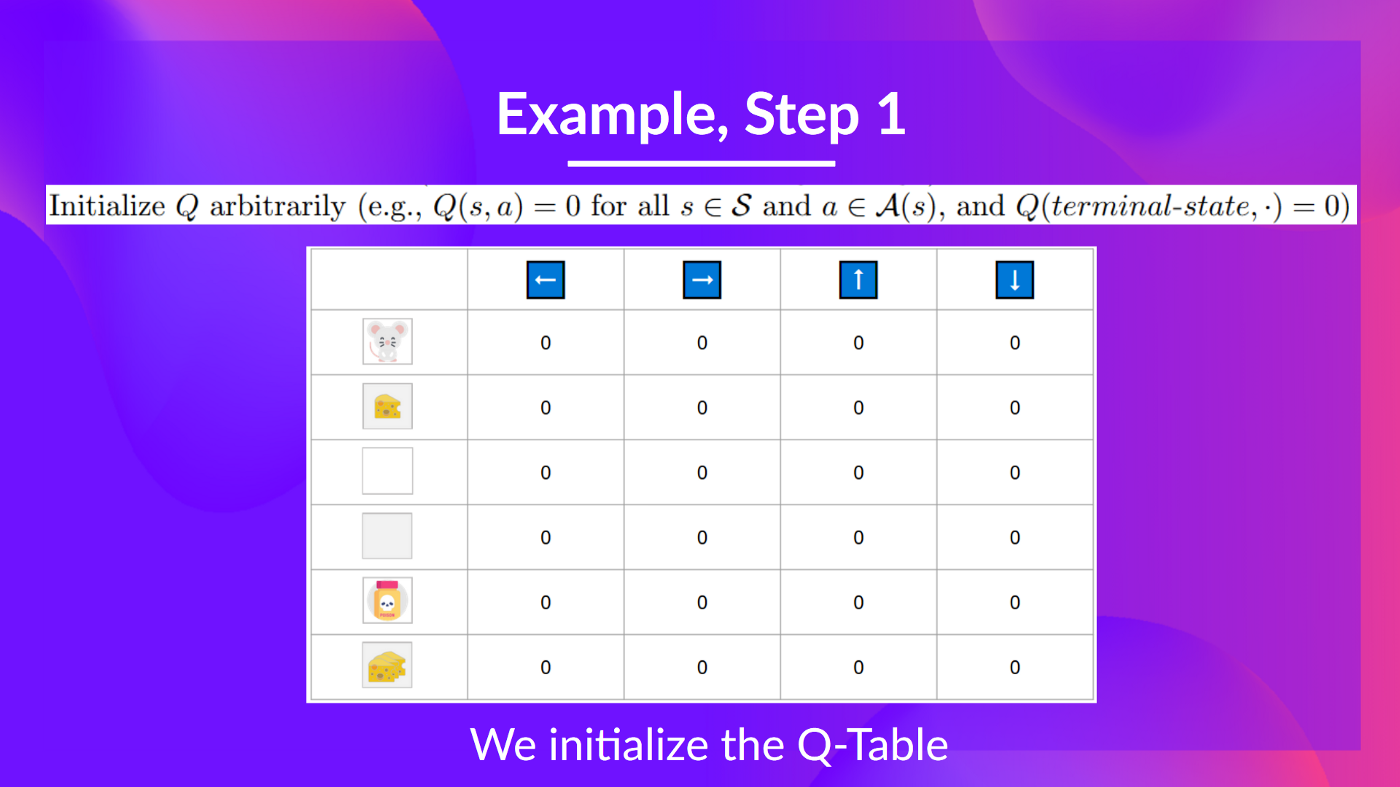
\includegraphics[width=0.6\linewidth,keepaspectratio]{rl117}
\end{center}

So, for now, our Q-Table is useless; we need to train our Q-function using the Q-Learning algorithm.

Let's do it for 2 training timesteps

{\tiny (Ref: Chapter 3 of the Deep Reinforcement Learning Class with Hugging Face)}

\end{frame}

%%%%%%%%%%%%%%%%%%%%%%%%%%%%%%%%%%%%%%%%%%%%%%%%%%%%%%%%%%%%%%%%%%%%%%%%%%%%%%%%%%
\begin{frame}[fragile]\frametitle{The Q-Learning Example}

Training timestep 1: Choose action using Epsilon Greedy Strategy. Because epsilon is big = 1.0, I take a random action, in this case, I go right.

\begin{center}
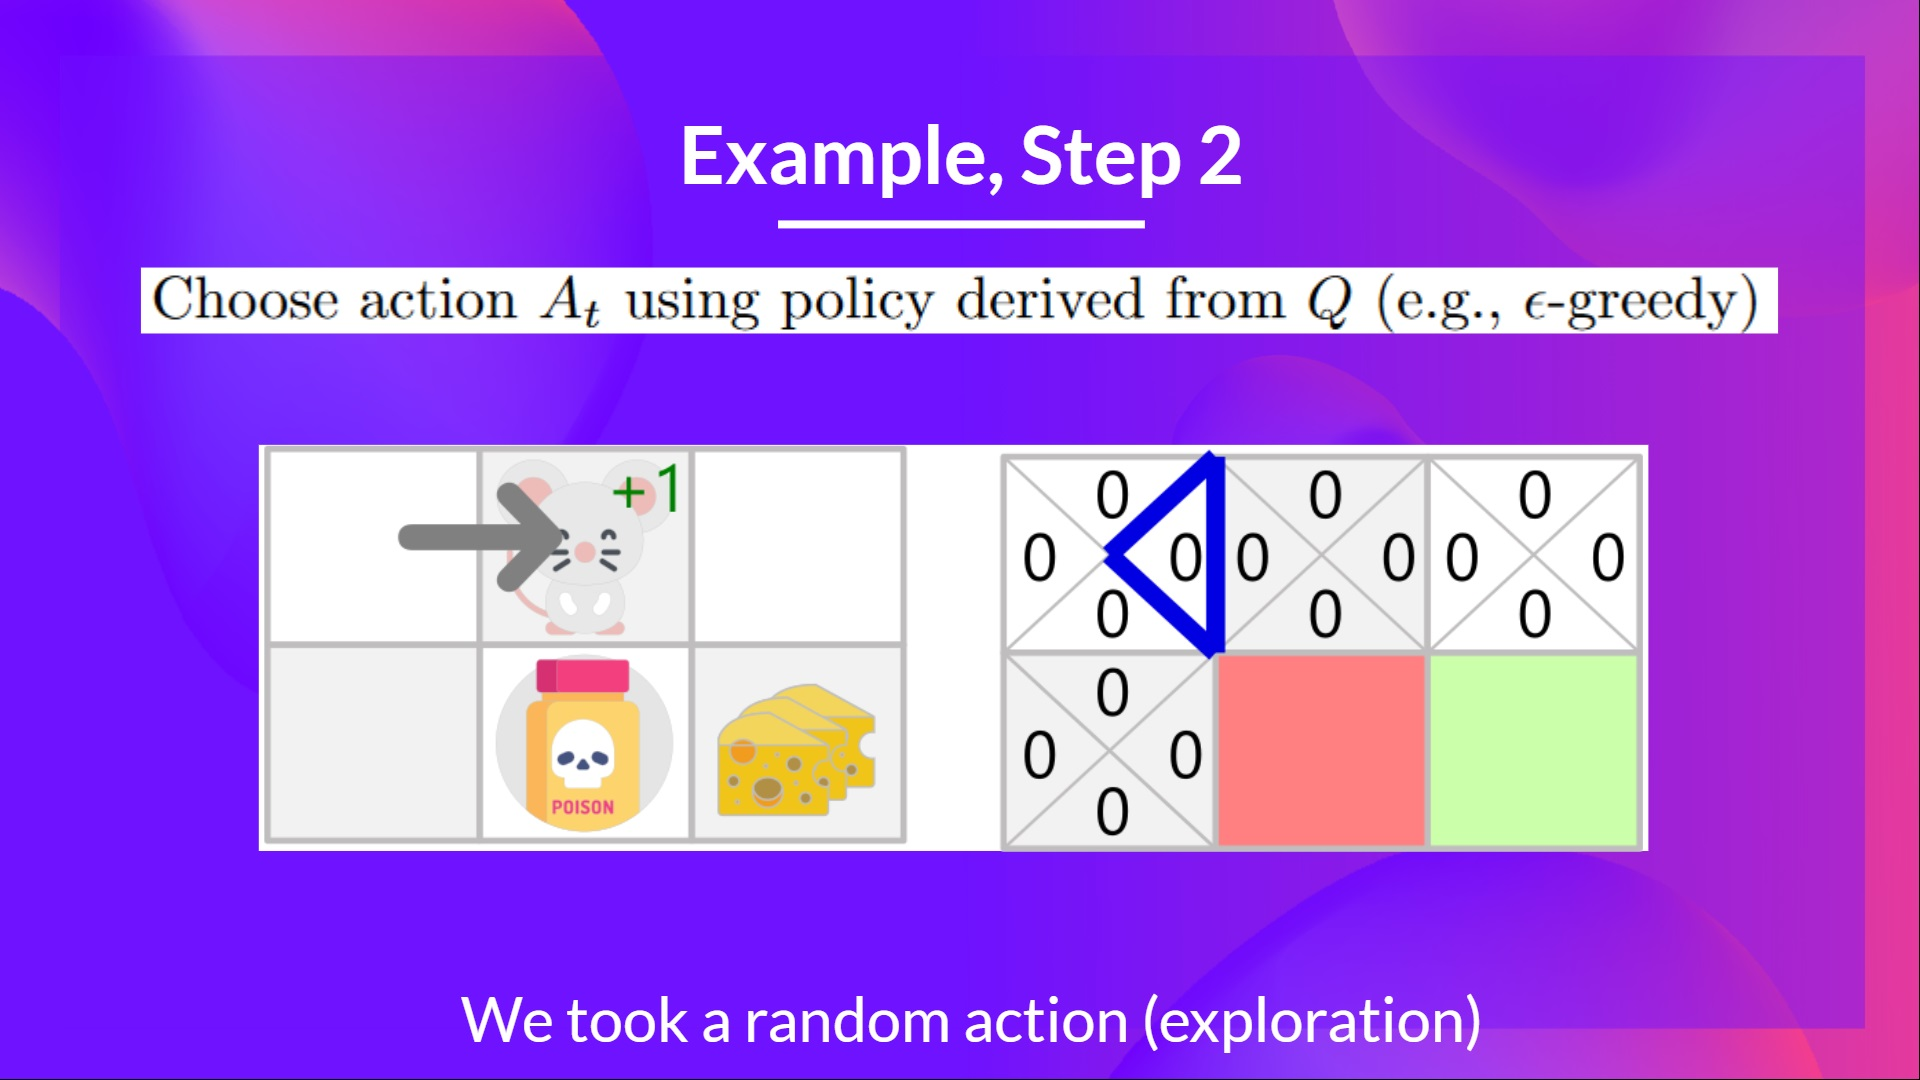
\includegraphics[width=0.6\linewidth,keepaspectratio]{rl118}
\end{center}

Perform action $A_t$, gets $R_{t+1}$ and $S_{t+1}$. By going right, I've got a small cheese, so $R_{t+1} = 1$, and I'm in a new state.

\begin{center}
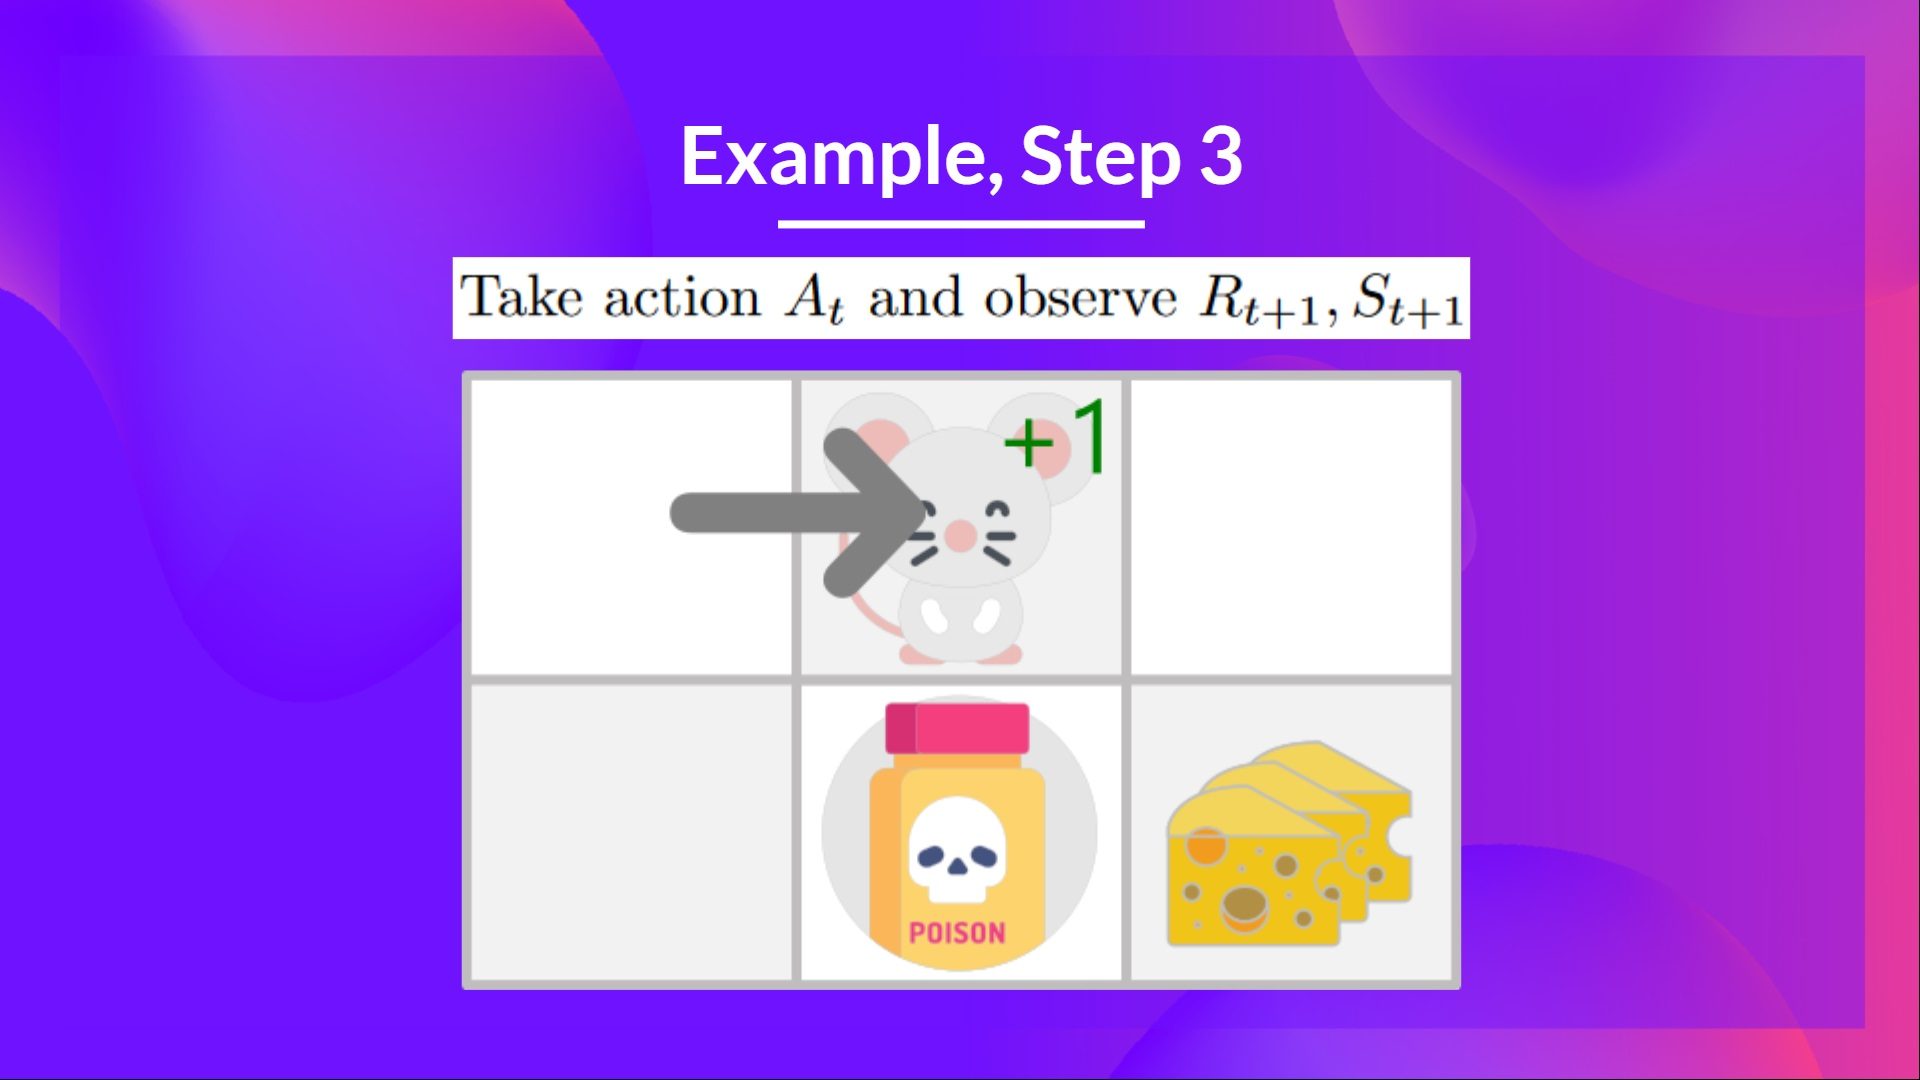
\includegraphics[width=0.6\linewidth,keepaspectratio]{rl119}
\end{center}

{\tiny (Ref: Chapter 3 of the Deep Reinforcement Learning Class with Hugging Face)}

\end{frame}


%%%%%%%%%%%%%%%%%%%%%%%%%%%%%%%%%%%%%%%%%%%%%%%%%%%%%%%%%%%%%%%%%%%%%%%%%%%%%%%%%%
\begin{frame}[fragile]\frametitle{The Q-Learning Example}

Update $Q(S_t, A_t)$

\begin{center}
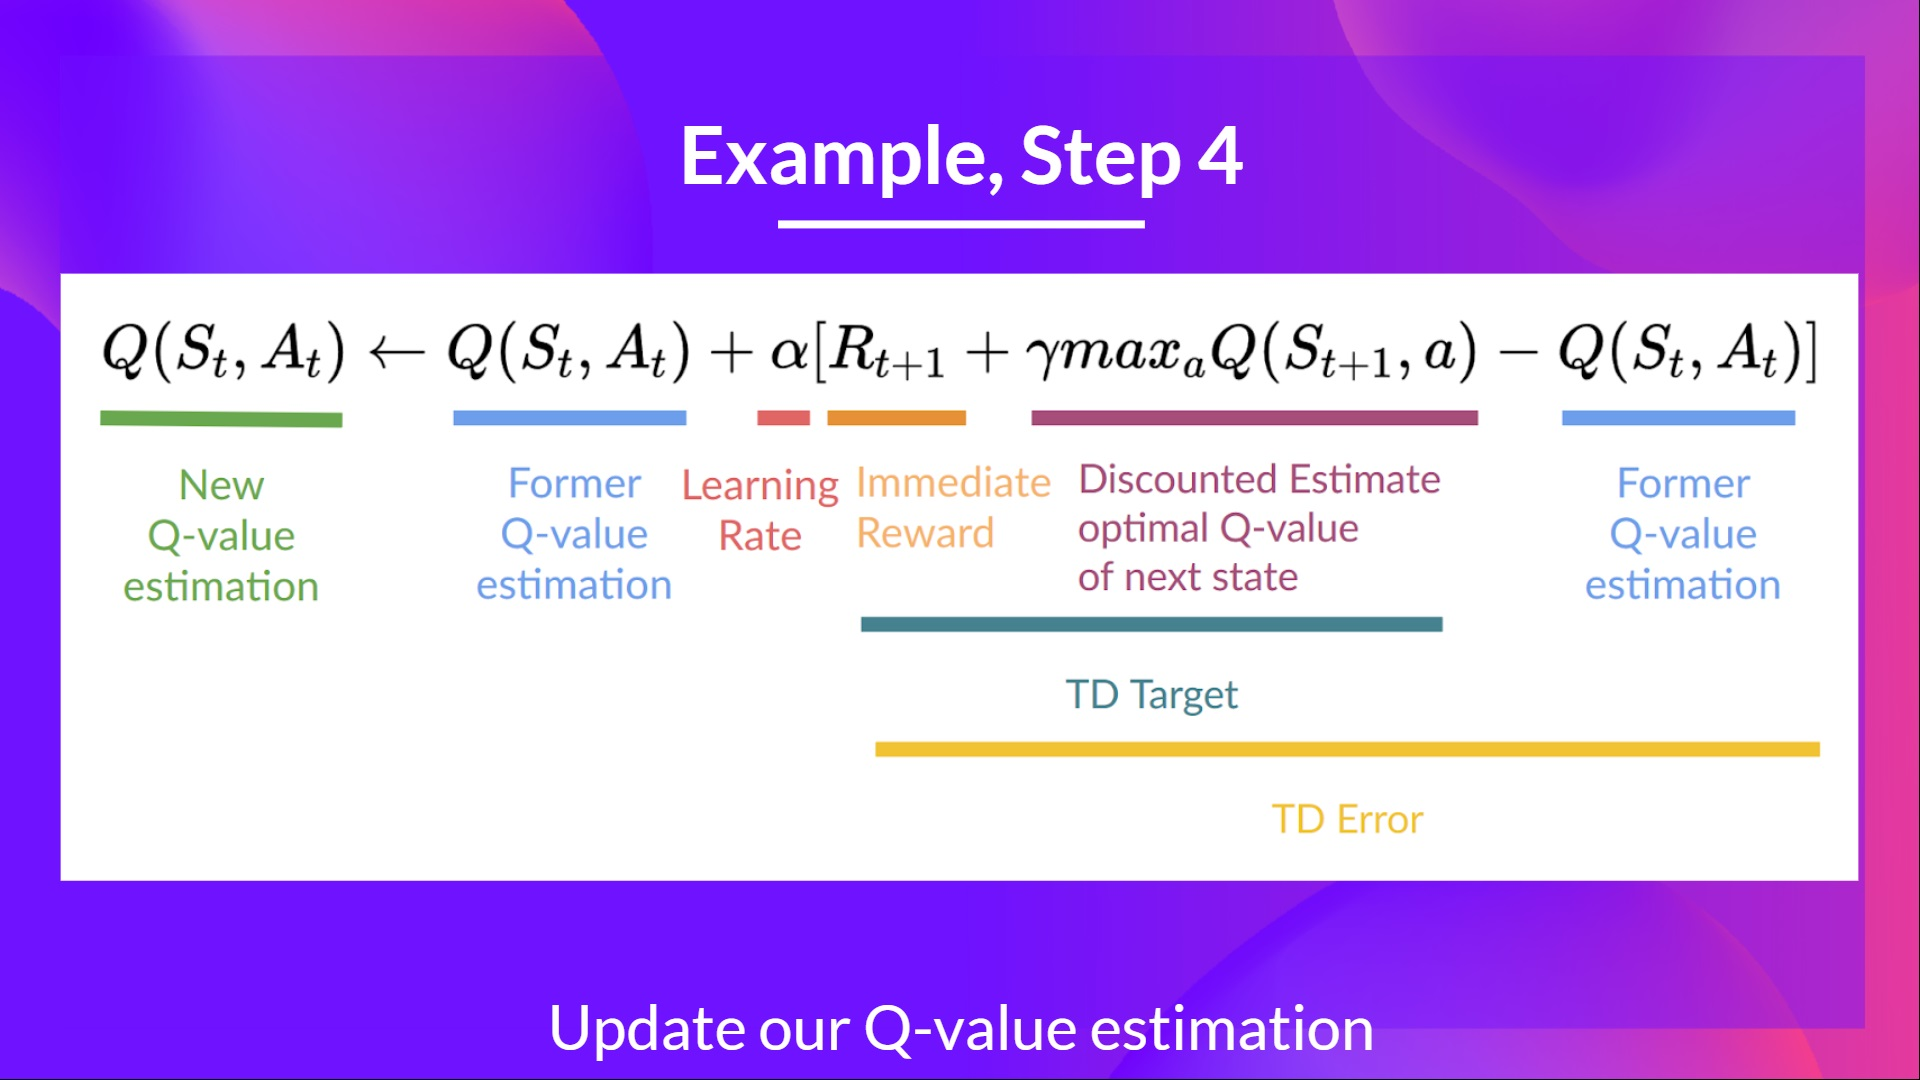
\includegraphics[width=0.6\linewidth,keepaspectratio]{rl120}

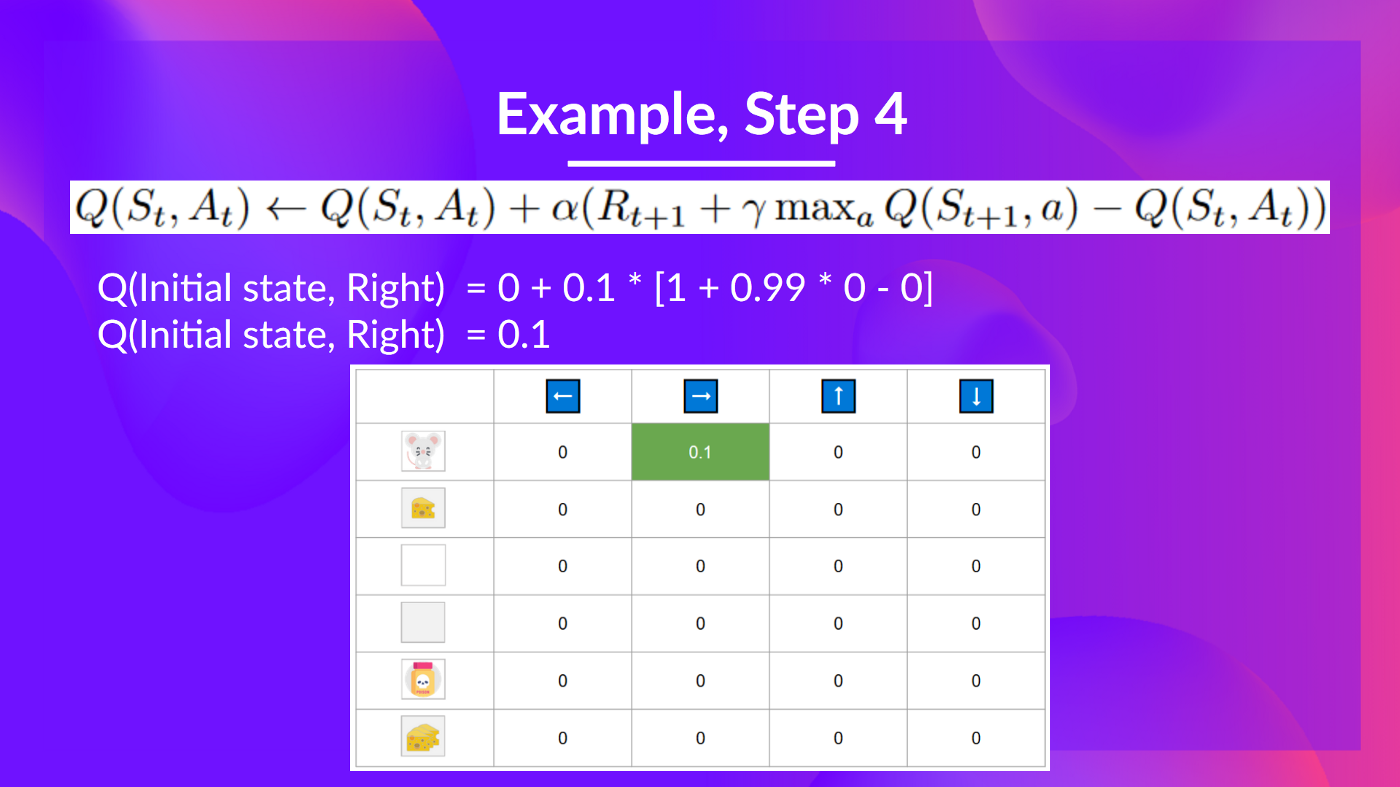
\includegraphics[width=0.6\linewidth,keepaspectratio]{rl121}

\end{center}


{\tiny (Ref: Chapter 3 of the Deep Reinforcement Learning Class with Hugging Face)}

\end{frame}



%%%%%%%%%%%%%%%%%%%%%%%%%%%%%%%%%%%%%%%%%%%%%%%%%%%%%%%%%%%%%%%%%%%%%%%%%%%%%%%%%%
\begin{frame}[fragile]\frametitle{The Q-Learning Example}

Training timestep 2: 

\begin{itemize}
\item Choose action using Epsilon Greedy Strategy
\item I take a random action again, since epsilon is big 0.99 (since we decay it a little bit because as the training progress, we want less and less exploration).
\item I took action down. Not a good action since it leads me to the poison
\end{itemize}

\begin{center}
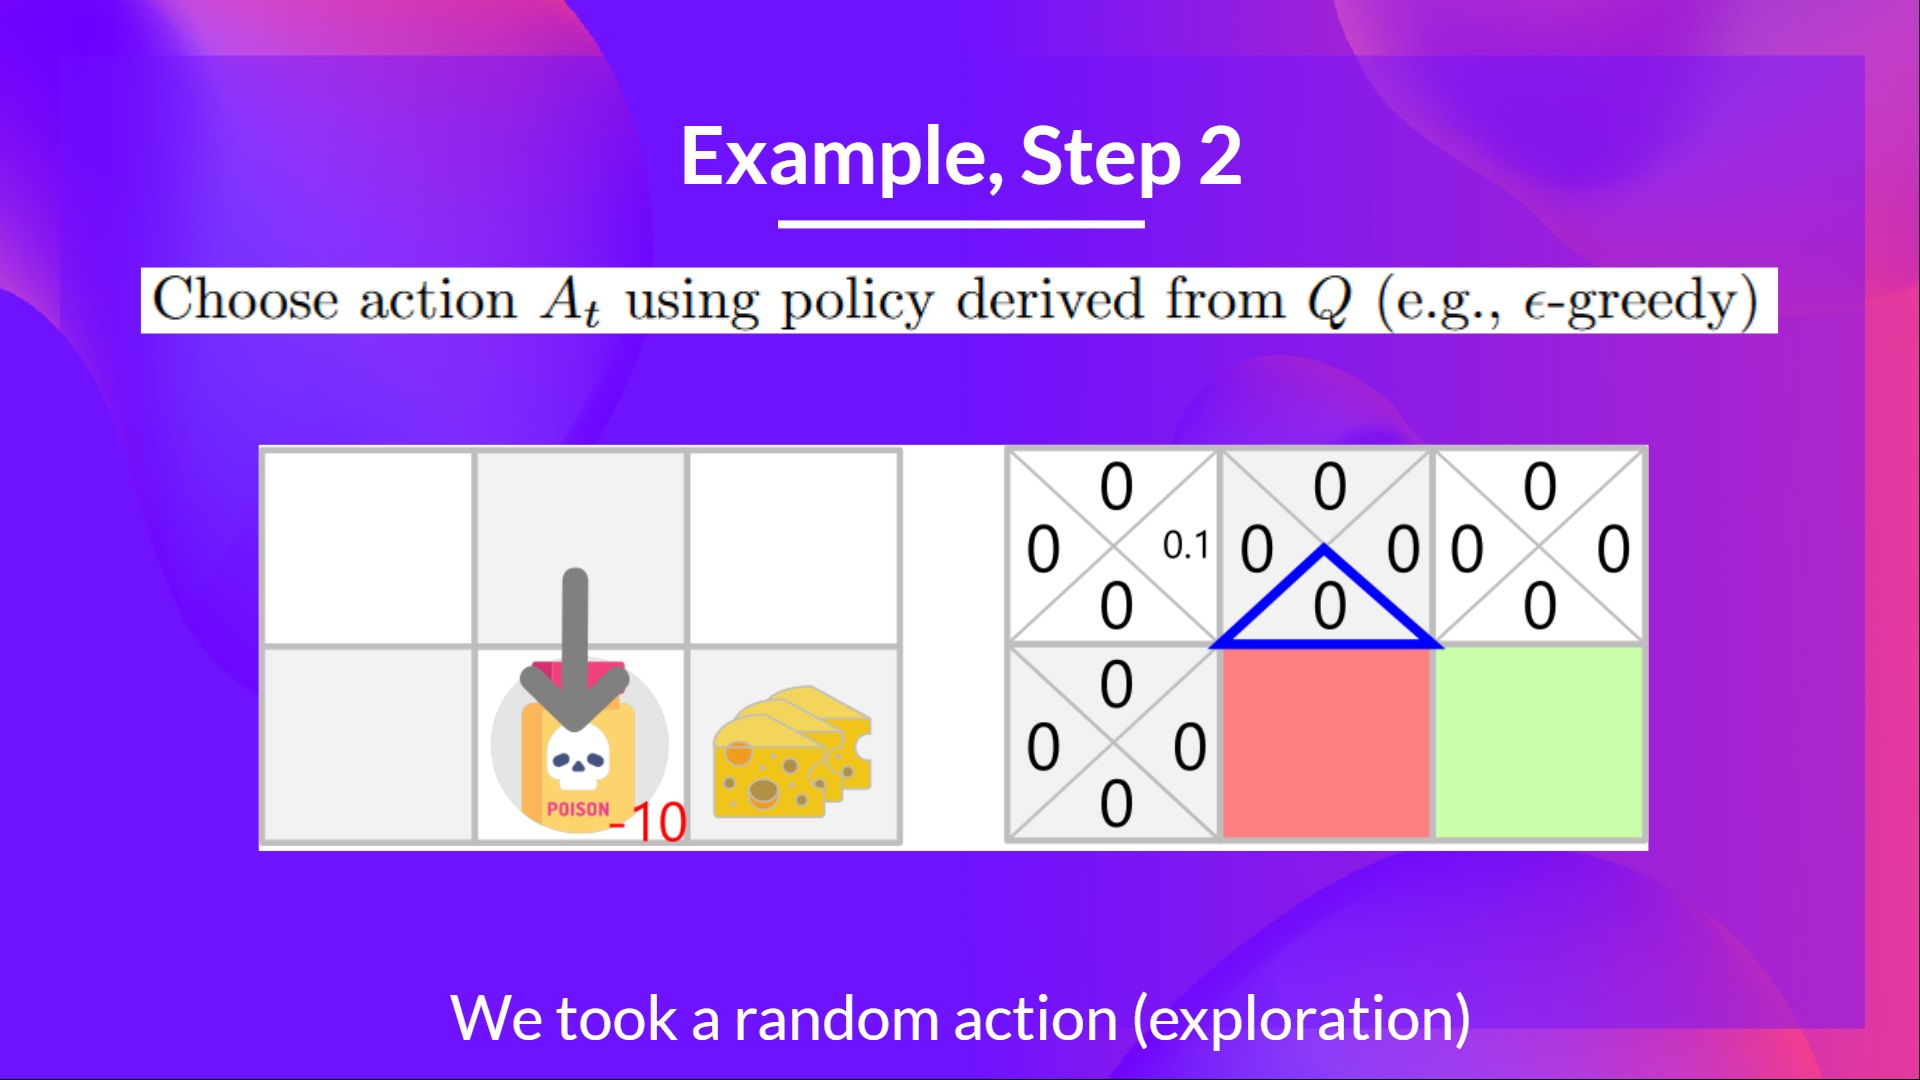
\includegraphics[width=0.6\linewidth,keepaspectratio]{rl122}

\end{center}


{\tiny (Ref: Chapter 3 of the Deep Reinforcement Learning Class with Hugging Face)}

\end{frame}

%%%%%%%%%%%%%%%%%%%%%%%%%%%%%%%%%%%%%%%%%%%%%%%%%%%%%%%%%%%%%%%%%%%%%%%%%%%%%%%%%%
\begin{frame}[fragile]\frametitle{The Q-Learning Example}

 Perform action At, gets $R_{t+1}$ and $S_{t+1}$. Because I go to the poison state, I get $R_{t+1} = -$, and I die.
 
\begin{center}
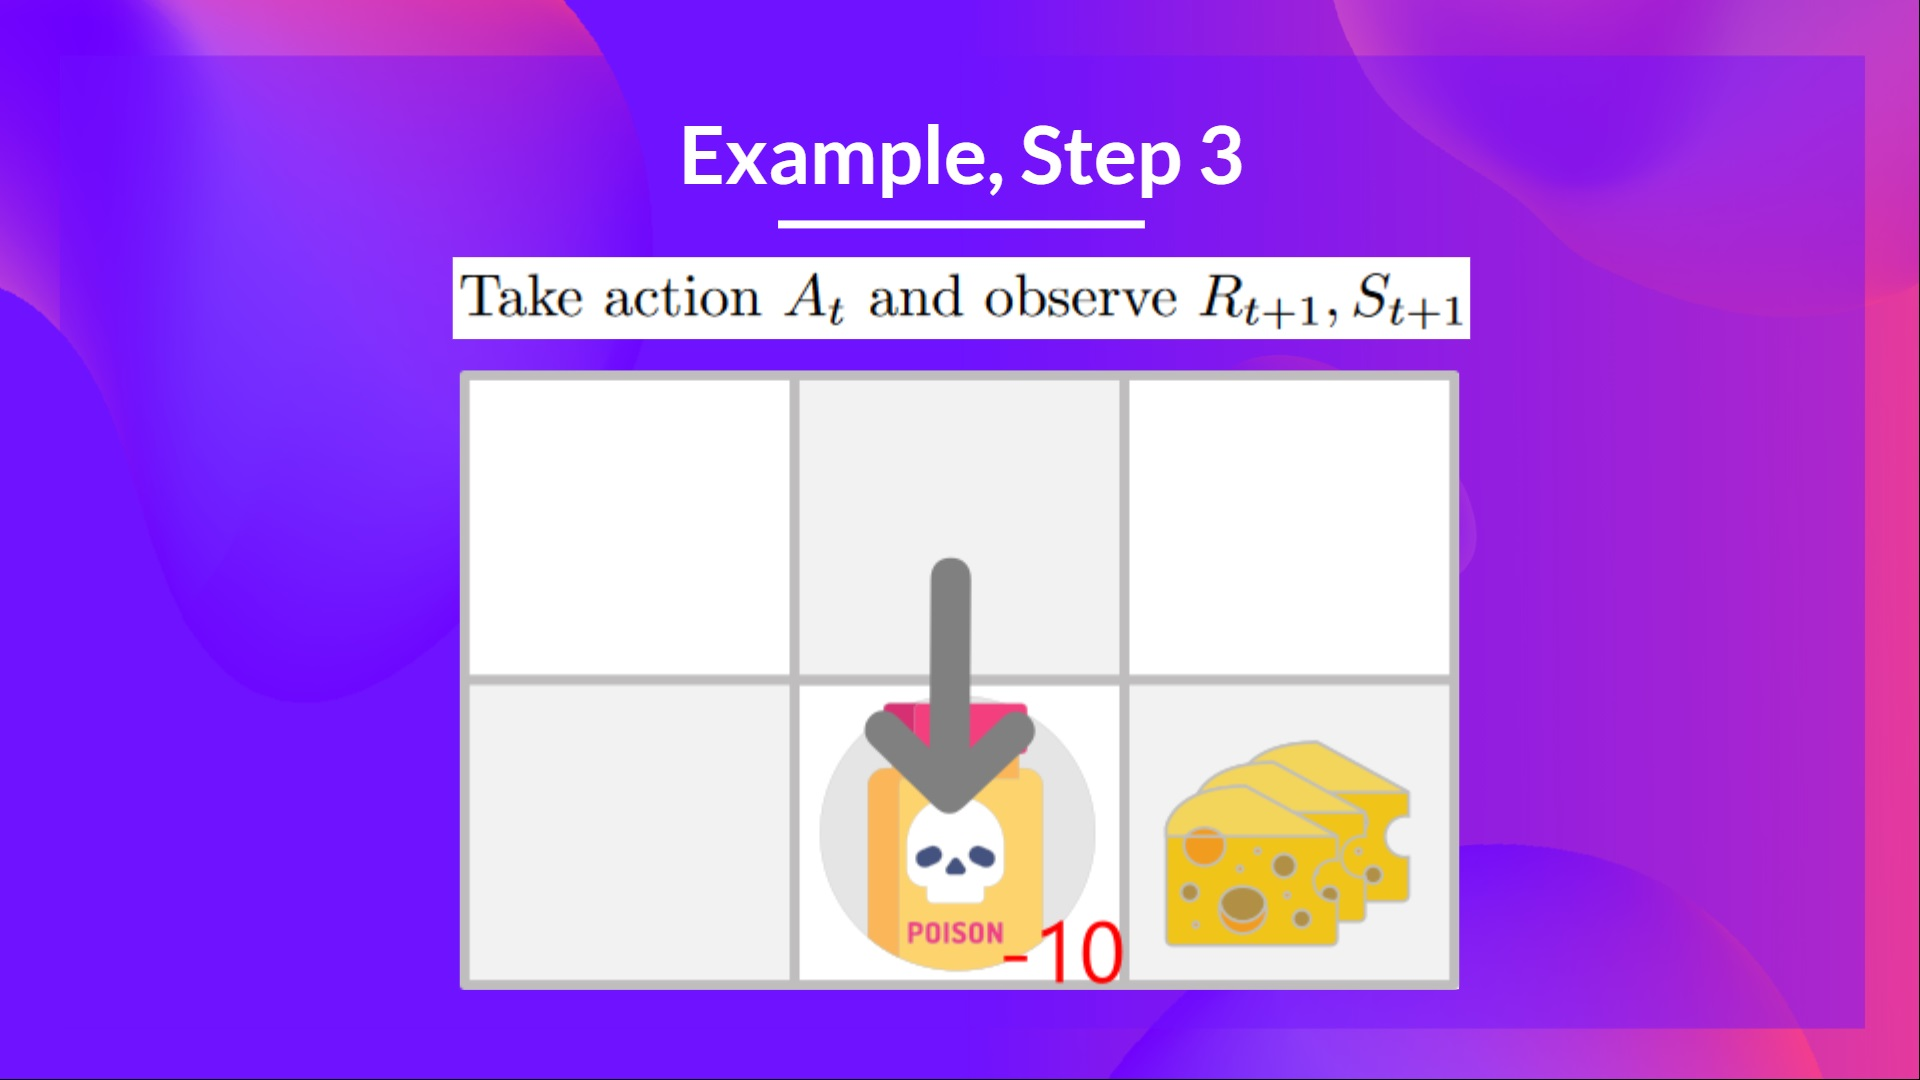
\includegraphics[width=0.6\linewidth,keepaspectratio]{rl123}

\end{center}


{\tiny (Ref: Chapter 3 of the Deep Reinforcement Learning Class with Hugging Face)}

\end{frame}

%%%%%%%%%%%%%%%%%%%%%%%%%%%%%%%%%%%%%%%%%%%%%%%%%%%%%%%%%%%%%%%%%%%%%%%%%%%%%%%%%%
\begin{frame}[fragile]\frametitle{The Q-Learning Example}

Update $Q(S_t, A_t)$

\begin{center}
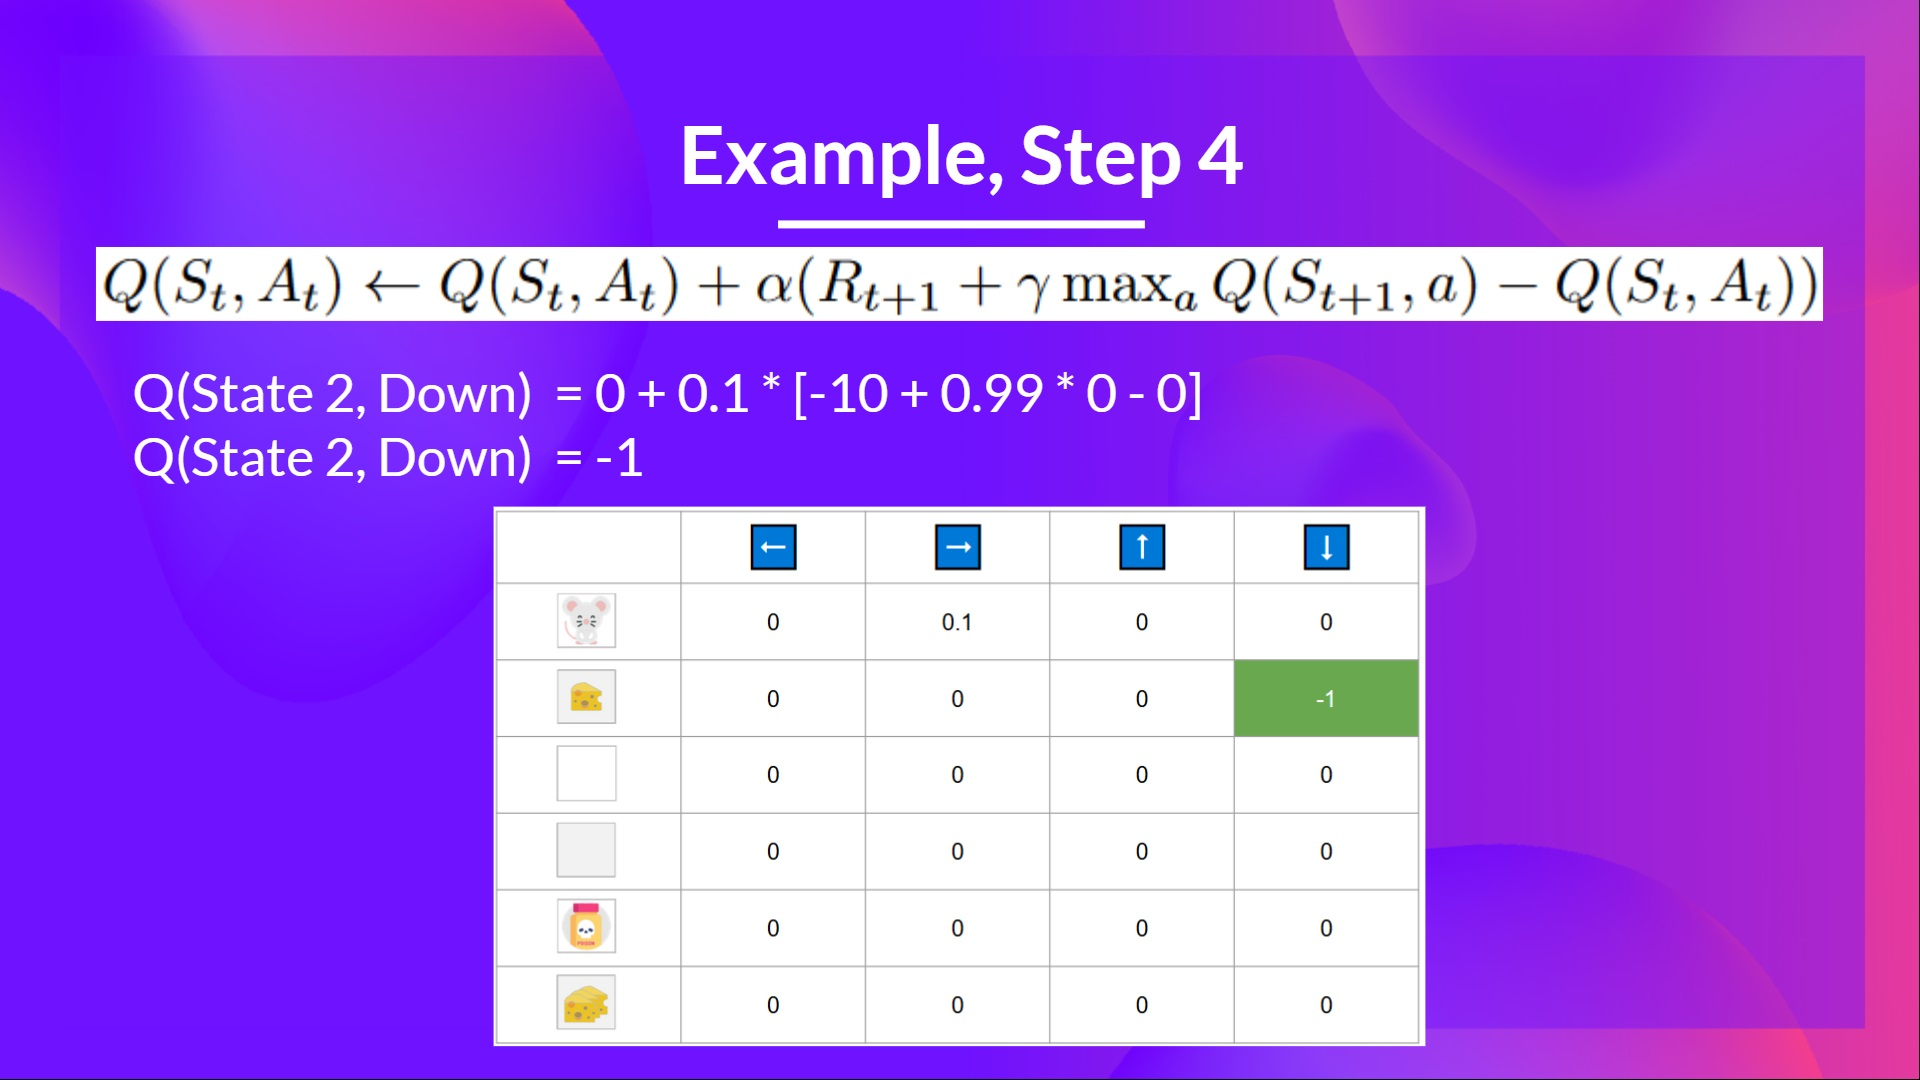
\includegraphics[width=0.6\linewidth,keepaspectratio]{rl124}

\end{center}

\begin{itemize}
\item Because we're dead, we start a new episode. But what we see here is that with two explorations steps, my agent became smarter.
\item As we continue exploring and exploiting the environment and updating Q-values using TD target, Q-Table will give us better and better approximations. And thus, at the end of the training, we'll get an optimal Q-Function.
\end{itemize}



{\tiny (Ref: Chapter 3 of the Deep Reinforcement Learning Class with Hugging Face)}

\end{frame}



%%%%%%%%%%%%%%%%%%%%%%%%%%%%%%%%%%%%%%%%%%%%%%%%%%%%%%%%%%%%%%%%%%%%%%%%%%%%%%%%%%
\begin{frame}[fragile]\frametitle{A Taxonomy of RL Algorithms}

\begin{center}
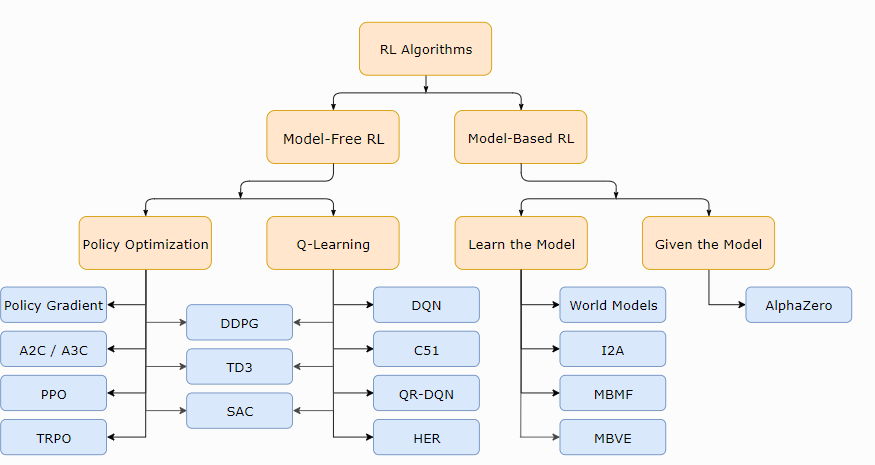
\includegraphics[width=\linewidth,keepaspectratio]{rl100}
\end{center}

{\tiny (Ref: Spinning Up - Open AI)}
\end{frame}

%%%%%%%%%%%%%%%%%%%%%%%%%%%%%%%%%%%%%%%%%%%%%%%%%%%%%%%%%%%%%%%%%%%%%%%%%%%%%%%%%%
\begin{frame}[fragile]\frametitle{Model-Free vs Model-Based RL}

\begin{itemize}
\item Core question: whether the agent has access to (or learns) a model of the environment. By a model of the environment, we mean a function which predicts state transitions and rewards.
\item Advantage of having model is that it allows the agent to plan by thinking ahead, seeing what would happen for a range of possible choices, and explicitly deciding between its options. Agents can then distill the results from planning ahead into a learned policy. A particularly famous example of this approach is AlphaZero. When this works, it can result in a substantial improvement in sample efficiency over methods that don’t have a model.
\item The main downside is that a ground-truth model of the environment is usually not available to the agent. 
\item If an agent wants to use a model in this case, it has to learn the model purely from experience, which creates several challenges. 

\end{itemize}

{\tiny (Ref: Spinning Up - Open AI)}
\end{frame}

%%%%%%%%%%%%%%%%%%%%%%%%%%%%%%%%%%%%%%%%%%%%%%%%%%%%%%%%%%%%%%%%%%%%%%%%%%%%%%%%%%
\begin{frame}[fragile]\frametitle{Model-Free vs Model-Based RL}

\begin{itemize}
\item The biggest challenge is that bias in the model can be exploited by the agent, resulting in an agent which performs well with respect to the learned model, but behaves sub-optimally (or super terribly) in the real environment. 
\item Model-learning is fundamentally hard, so even intense effort—being willing to throw lots of time and compute at it—can fail to pay off.
\item Algorithms which use a model are called model-based methods, and those that don’t are called model-free. 
\item While model-free methods forego the potential gains in sample efficiency from using a model, they tend to be easier to implement and tune.
\end{itemize}

{\tiny (Ref: Spinning Up - Open AI)}
\end{frame}

%%%%%%%%%%%%%%%%%%%%%%%%%%%%%%%%%%%%%%%%%%%%%%%%%%%%%%%%%%%%%%%%%%%%%%%%%%%%%%%%%%
\begin{frame}[fragile]\frametitle{What to Learn}

Another critical branching point in an RL algorithm is the question of what to learn. The list of usual suspects includes


\begin{itemize}
\item policies, either stochastic or deterministic,
\item action-value functions (Q-functions),
\item value functions,
\item and/or environment models.
\end{itemize}

{\tiny (Ref: Spinning Up - Open AI)}
\end{frame}

%%%%%%%%%%%%%%%%%%%%%%%%%%%%%%%%%%%%%%%%%%%%%%%%%%%%%%%%%%%%%%%%%%%%%%%%%%%%%%%%%%
\begin{frame}[fragile]\frametitle{Goal}

The goal in RL is to learn a policy which maximizes expected return. The optimal policy $\pi^*$ is:
%
\begin{equation*}
\pi^* = \arg \max_{\pi} E_{\tau \sim \pi}[R(\tau)],
\end{equation*}
%
where by $\tau \sim \pi$, we mean
%
\begin{equation*}
s_0 \sim \mu(\cdot), \;\;\;\;\; a_t \sim \pi(\cdot|s_t), \;\;\;\;\; s_{t+1} \sim P(\cdot | s_t, a_t).
\end{equation*}


There are two main approaches for solving this problem:
\begin{itemize}
\item policy optimization
\item and Q-learning.
\end{itemize}


{\tiny (Ref: Intro to RL - Joshua Achiam)}


\end{frame}

%%%%%%%%%%%%%%%%%%%%%%%%%%%%%%%%%%%%%%%%%%%%%%%%%%%%%%%%%%%%%%%%%%%%%%%%%%%%%%%%%%
\begin{frame}[fragile]\frametitle{Q-Learning}

\begin{itemize}
\item Core idea: learn $Q^*$ and use it to get the optimal actions
\item Way to do it:
\begin{itemize}
\item Collect experience in the environment using a policy which trades off between acting randomly and acting according to current $Q_{\theta}$
\item Interleave data collection with updates to $Q_{\theta}$ to minimize Bellman error:
%
\begin{equation*}
\min_{\theta} \sum_{(s,a,s',r)\in D} \left(Q_{\theta}(s,a) - \left(r + \gamma \max_{a'} Q_{\theta}(s',a') \right) \right)^2
\end{equation*}
...sort of! This actually won't work!
\end{itemize}

\end{itemize}
{\tiny (Ref: Intro to RL - Joshua Achiam)}


\end{frame}


%%%%%%%%%%%%%%%%%%%%%%%%%%%%%%%%%%%%%%%%%%%%%%%%%%%%%%%%%%%%%%%%%%%%%%%%%%%%%%%%%%
\begin{frame}[fragile]\frametitle{What to Learn in Model-Free RL}

There are two main approaches to representing and training agents with model-free RL:

\begin{itemize}
\item Policy Optimization. Methods in this family represent a policy explicitly as $\pi_{\theta}(a|s)$. They optimize the parameters $\theta$ either directly by gradient ascent on the performance objective $J(\pi_{\theta})$, or indirectly, by maximizing local approximations of $J(\pi_{\theta})$. 
\item  almost always performed on-policy, which means that each update only uses data collected while acting according to the most recent version of the policy.
\item E.g A2C/A3C, PPO
\item Q-Learning. Methods in this family learn an approximator $Q_{\theta}(s,a)$ for the optimal action-value function,$ Q^*(s,a)$. Typically they use an objective function based on the Bellman equation.
\item almost always performed off-policy, which means that each update can use data collected at any point during training, regardless of how the agent was choosing to explore the environment when the data was obtained. 
\item E.g. DQN, C51
\end{itemize}

{\tiny (Ref: Spinning Up - Open AI)}
\end{frame}

%%%%%%%%%%%%%%%%%%%%%%%%%%%%%%%%%%%%%%%%%%%%%%%%%%%%%%%%%%%%%%%%%%%%%%%%%%%%%%%%%%
\begin{frame}[fragile]\frametitle{Trade-offs}

Trade-offs Between Policy Optimization and Q-Learning. 

\begin{itemize}
\item Policy Optimization. you directly optimize for the thing you want. This tends to make them stable and reliable. 
\item Q-Learning. indirectly optimize for agent performance, by training $Q_{\theta}$ to satisfy a self-consistency equation. There are many failure modes for this kind of learning, so it tends to be less stable
\item But, Q-learning methods gain the advantage of being substantially more sample efficient when they do work, because they can reuse data more effectively than policy optimization techniques.
\end{itemize}

{\tiny (Ref: Spinning Up - Open AI)}
\end{frame}

%%%%%%%%%%%%%%%%%%%%%%%%%%%%%%%%%%%%%%%%%%%%%%%%%%%%%%%%%%%%%%%%%%%%%%%%%%%%%%%%%%
\begin{frame}[fragile]\frametitle{Interpolating }

Interpolating Between Policy Optimization and Q-Learning

\begin{itemize}
\item policy optimization and Q-learning are not incompatible
\item Algorithms that live on this spectrum are able to carefully trade-off between the strengths and weaknesses of either side.
\item Examples:
\begin{itemize}
\item DDPG, an algorithm which concurrently learns a deterministic policy and a Q-function by using each to improve the other,
\item and SAC, a variant which uses stochastic policies, entropy regularization, and a few other tricks to stabilize learning and score higher than DDPG on standard benchmarks.
\end{itemize}

\end{itemize}

{\tiny (Ref: Spinning Up - Open AI)}
\end{frame}

%%%%%%%%%%%%%%%%%%%%%%%%%%%%%%%%%%%%%%%%%%%%%%%%%%%%%%%%%%%%%%%%%%%%%%%%%%%%%%%%%%
\begin{frame}[fragile]\frametitle{What to Learn in Model-Based RL}

Unlike model-free RL, there aren’t a small number of easy-to-define clusters of methods for model-based RL: there are many orthogonal ways of using models.  In each case, the model may either be given or learned.

\begin{itemize}
\item Background: Pure Planning. The most basic approach never explicitly represents the policy, and instead, uses pure planning techniques like model-predictive control (MPC) to select actions. E.g. The MBMF work explores MPC with learned environment models on some standard benchmark tasks for deep RL.
\item Expert Iteration. A straightforward follow-on to pure planning involves using and learning an explicit representation of the policy, $\pi_{\theta}(a|s)$. The agent uses a planning algorithm (like Monte Carlo Tree Search) in the model, generating candidate actions for the plan by sampling from its current policy. E.g. Exlt, Alpha Zero.
\item Data Augmentation for Model-Free Methods. Use a model-free RL algorithm to train a policy or Q-function, but either with Real+fictitious experience or just fictitious. E.g. MBVE.
\item Embedding Planning Loops into Policies. Another approach embeds the planning procedure directly into a policy as a subroutine—so that complete plans become side information for the policy—while training the output of the policy with any standard model-free algorithm. E.g. I2A.
\end{itemize}

{\tiny (Ref: Spinning Up - Open AI)}
\end{frame}

%%%%%%%%%%%%%%%%%%%%%%%%%%%%%%%%%%%%%%%%%%%%%%%%%%%%%%%%%%%%%%%%%%%%%%%%%%%%%%%%%%
\begin{frame}[fragile]\frametitle{Deriving the Simplest Policy Gradient}

\begin{itemize}
\item Consider the case of a stochastic, parameterized policy, $\pi_{\theta}$. 
\item Aim to maximize the expected return $J(\pi_{\theta}) = E_{\tau \sim \pi_{\theta}}[R(\tau)]$.
\item optimize the policy by gradient ascent, eg $\theta_{k+1} = \theta_k + \alpha \left. \nabla_{\theta} J(\pi_{\theta}) \right|_{\theta_k}.$ 
\item The gradient of policy performance, $\nabla_{\theta} J(\pi_{\theta})$, is called the policy gradient, and algorithms that optimize the policy this way are called policy gradient algorithms. (Examples include Vanilla Policy Gradient and TRPO. PPO is often referred to as a policy gradient algorithm, though this is slightly inaccurate.)
\item To actually use this algorithm, we need an expression for the policy gradient which we can numerically compute. This involves two steps:
\begin{itemize}
\item deriving the analytical gradient of policy performance, which turns out to have the form of an expected value, and then 
\item forming a sample estimate of that expected value, which can be computed with data from a finite number of agent-environment interaction steps.
\end{itemize}
\end{itemize}

{\tiny (Ref: Spinning Up - Open AI)}
\end{frame}

%%%%%%%%%%%%%%%%%%%%%%%%%%%%%%%%%%%%%%%%%%%%%%%%%%%%%%%%%%%%%%%%%%%%%%%%%%%%%%%%%%
\begin{frame}[fragile]\frametitle{Deriving the Simplest Policy Gradient}

Terms used
\begin{itemize}
\item  Probability of a Trajectory. The probability of a trajectory $\tau = (s_0, a_0, ..., s_{T+1})$ given that actions come from $\pi_{\theta}$ is

$P(\tau|\theta) = \rho_0 (s_0) \prod_{t=0}^{T} P(s_{t+1}|s_t, a_t) \pi_{\theta}(a_t |s_t)$.
\item  The Log-Derivative Trick is based on a simple rule from calculus: the derivative of $\log x$ with respect to x is 1/x. When rearranged and combined with chain rule, we get:$ \nabla_{\theta} P(\tau | \theta) = P(\tau | \theta) \nabla_{\theta} \log P(\tau | \theta)$.
\item Log-Probability of a Trajectory. The log-prob of a trajectory is just $\log P(\tau|\theta) = \log \rho_0 (s_0) + \sum_{t=0}^{T} \bigg( \log P(s_{t+1}|s_t, a_t)  + \log \pi_{\theta}(a_t |s_t)\bigg)$.
\end{itemize}

{\tiny (Ref: Spinning Up - Open AI)}
\end{frame}

%%%%%%%%%%%%%%%%%%%%%%%%%%%%%%%%%%%%%%%%%%%%%%%%%%%%%%%%%%%%%%%%%%%%%%%%%%%%%%%%%%
\begin{frame}[fragile]\frametitle{Deriving the Simplest Policy Gradient}

Terms used
\begin{itemize}
\item   Gradients of Environment Functions. The environment has no dependence on $\theta$, so gradients of $\rho_0(s_0), P(s_{t+1}|s_t, a_t)$, and $R(\tau)$ are zero.
\item  Grad-Log-Prob of a Trajectory. The gradient of the log-prob of a trajectory is thus

\end{itemize}

% \begin{align*}
% \nabla_{\theta} \log P(\tau | \theta) &= \cancel{\nabla_{\theta} \log \rho_0 (s_0)} + \sum_{t=0}^{T} \bigg( \cancel{\nabla_{\theta} \log P(s_{t+1}|s_t, a_t)}  + \nabla_{\theta} \log \pi_{\theta}(a_t |s_t)\bigg) \\
% &= \sum_{t=0}^{T} \nabla_{\theta} \log \pi_{\theta}(a_t |s_t)
% \end{align*}


{\tiny (Ref: Spinning Up - Open AI)}
\end{frame}

%%%%%%%%%%%%%%%%%%%%%%%%%%%%%%%%%%%%%%%%%%%%%%%%%%%%%%%%%%%%%%%%%%%%%%%%%%%%%%%%%%
\begin{frame}[fragile]\frametitle{Putting it all together}

\begin{align*}
\nabla_{\theta} J(\pi_{\theta}) &= \nabla_{\theta} E_{\tau \sim \pi_{\theta}}[R(\tau)] & \\
&= \nabla_{\theta} \int_{\tau} P(\tau|\theta) R(\tau) & \text{Expand expectation} \\
&= \int_{\tau} \nabla_{\theta} P(\tau|\theta) R(\tau) & \text{Bring gradient under integral} \\
&= \int_{\tau} P(\tau|\theta) \nabla_{\theta} \log P(\tau|\theta) R(\tau) & \text{Log-derivative trick} \\
&= E_{\tau \sim \pi_{\theta}}{\nabla_{\theta} \log P(\tau|\theta) R(\tau)} & \text{Return to expectation form} \\
\therefore \nabla_{\theta} J(\pi_{\theta}) &= E_{\tau \sim \pi_{\theta}}{\sum_{t=0}^{T} \nabla_{\theta} \log \pi_{\theta}(a_t |s_t) R(\tau)} & \text{Expression for grad-log-prob}
\end{align*}

This is an expectation, which means that we can estimate it with a sample mean.


{\tiny (Ref: Spinning Up - Open AI)}
\end{frame}

%%%%%%%%%%%%%%%%%%%%%%%%%%%%%%%%%%%%%%%%%%%%%%%%%%%%%%%%%%%%%%%%%%%%%%%%%%%%%%%%%%
\begin{frame}[fragile]\frametitle{Putting it all together}

If we collect a set of trajectories $\mathcal{D} = \{\tau_i\}_{i=1,...,N}$ where each trajectory is obtained by letting the agent act in the environment using the policy $\pi_{\theta}$, the policy gradient can be estimated with

$\hat{g} = \frac{1}{|\mathcal{D}|} \sum_{\tau \in \mathcal{D}} \sum_{t=0}^{T} \nabla_{\theta} \log \pi_{\theta}(a_t |s_t) R(\tau)$,

where $|\mathcal{D}|$ is the number of trajectories in $\mathcal{D}$ (here, $N$).

This last expression is the simplest version of the computable expression. Assuming that we have represented our policy in a way which allows us to calculate $\nabla_{\theta} \log \pi_{\theta}(a|s)$, and if we are able to run the policy in the environment to collect the trajectory dataset, we can compute the policy gradient and take an update step.

{\tiny (Ref: Spinning Up - Open AI)}
\end{frame}



%%%%%%%%%%%%%%%%%%%%%%%%%%%%%%%%%%%%%%%%%%%%%%%%%%%%%%%%%%%%%%%%%%%%%%%%%%%%%%%%%%
\begin{frame}[fragile]\frametitle{Q Learning Algorithm}

\begin{itemize}
\item Initialize Q for all states s and actions a 
\item Initialize $\alpha=0.001,\gamma=0.9,\epsilon_{max}=1.0,\epsilon_{min}=0.01$
\item Repeat for n\_episodes
	\begin{itemize}
	\item Initialize state s 
	\item For each step of episode
		\begin{itemize}
		\item Choose a with epsilon-greedy 
		\item Perform a, get new state s’ and reward r 
		\item $Q(s ,a)=Q(s,a)+ \alpha (r + \gamma max Q(s' ,a_{max})- Q(s ,a))$
		\item s = s'
		\end{itemize}
	\end{itemize}
\end{itemize}

{\tiny (Ref: Modern Reinforcement Learning: Deep Q Learning in PyTorch - Phil Tabor)}

\end{frame}